\documentclass[journal]{IEEEtran}

\usepackage{amsmath,amssymb,amsfonts}
\usepackage{graphicx}
\usepackage{textcomp}
\usepackage{xcolor}
\usepackage{booktabs}
\usepackage{colortbl}
\usepackage{multirow}
\usepackage{url}
\usepackage{xurl}
\usepackage{float}
\usepackage{cite}
\usepackage{mdframed}
\usepackage{tikz}
\usepackage{pgfplots}
\usetikzlibrary{arrows.meta,positioning,shapes.geometric,fit,calc,backgrounds}
\pgfplotsset{compat=1.18}
\usepackage{hyperref}

% ── Color definitions (Rule Q) ──────────────────────────────────────────────
\definecolor{darkblue}{RGB}{0,0,139}
\definecolor{midgreen}{RGB}{34,139,34}
\definecolor{deepred}{RGB}{180,0,0}
\definecolor{steelblue}{RGB}{52,102,153}
\definecolor{tealcolor}{RGB}{0,110,110}
\definecolor{ambercolor}{RGB}{204,102,0}
\definecolor{slateblue}{RGB}{90,80,160}

% ── Framework name (single point of change) ─────────────────────────────────
\newcommand{\hacof}{HACOF}

% ── Suppress IEEEtran's hardcoded Abstract/Keywords labels ──────────────────
\makeatletter
\def\abstract{\normalfont
    \if@twocolumn
      \relax
    \else
      \bgroup\par\addvspace{0.5\baselineskip}\centering\vspace{-1.78ex}%
      \@IEEEabskeysecsize\textbf{\abstractname}%
      \par\addvspace{0.5\baselineskip}\egroup\quotation\@IEEEabskeysecsize
    \fi\@IEEEgobbleleadPARNLSP}
\def\IEEEkeywords{\normalfont
    \if@twocolumn
      \relax
    \else
      \bgroup\par\addvspace{0.5\baselineskip}\centering\@IEEEabskeysecsize%
      \textbf{\IEEEkeywordsname}%
      \par\addvspace{0.5\baselineskip}\egroup\quotation\@IEEEabskeysecsize
    \fi\@IEEEgobbleleadPARNLSP}
\makeatother

\hypersetup{colorlinks=true,linkcolor=darkblue,citecolor=darkblue,urlcolor=darkblue}

\begin{document}

\title{\textcolor{darkblue}{Law, Policy, and Governance of the AI Ecosystem for Human Control: The Human-Centric AI Governance and Continuous Oversight Framework (HACOF)}}

\author{%
  \IEEEauthorblockN{\textcolor{slateblue}{\itshape Muhammad Faisal Laiq
    \qquad Email:~shmlaiq@gmail.com \qquad
    ORCID:~0009-0007-5779-9836}}%
}

\maketitle

\begin{abstract}
\begin{mdframed}[
  linecolor=darkblue, linewidth=1.8pt,
  backgroundcolor=darkblue!5,
  innerleftmargin=10pt, innerrightmargin=10pt,
  innertopmargin=9pt, innerbottommargin=9pt,
  roundcorner=5pt, skipabove=0pt, skipbelow=0pt
]
\noindent\textbf{\textcolor{darkblue}{Abstract\,---}}~Artificial intelligence (AI) systems, autonomous agents, and intelligent bots act faster than human supervisors can inspect them. We propose the Human-Centric AI Governance and Continuous Oversight Framework (HACOF), an integrated model combining legally enforceable AI policies, technical safety controls, independent supervisory AI agents, real-time behavioral monitoring, automated containment mechanisms, and accountable human governance. AI systems operate within explicitly defined legal, ethical, operational, and technical boundaries, while dedicated supervisory agents continuously evaluate AI activities, identify policy violations, detect emerging risks, and initiate proportionate protective actions. Authority flows from human rights and law, through institutional policy and technical guardrails, to supervisory agents that monitor compliance across the AI lifecycle and are themselves governed; high-risk violations trigger immediate containment, and ambiguous or consequential decisions go to authorized human reviewers. Because absolute prevention cannot be guaranteed, HACOF rests on defense-in-depth, independent verification, resilience, and continuous improvement, aiming to reduce the likelihood, severity, and duration of harm while preserving innovation, autonomy, privacy, and due process. We decompose the state capacity to require and verify such oversight into four pillars: boundary-setting, incentive-steering, human-in-the-loop (HITL) regulatory capacity, and algorithmic auditing access. All four concentrate in the United States, European Union, and China. We use Pakistan's 2025 National AI Policy to show what a low-capacity state can mandate. A prototype passes its self-tests, and in a simulation with assumed detector rates HACOF cuts residual harm about elevenfold versus a baseline. As a policy-oriented reference model, HACOF integrates established runtime-enforcement and AI-control techniques into an enforceable, auditable, contestable form.
\end{mdframed}
\end{abstract}

\begin{IEEEkeywords}
\begin{mdframed}[
  linecolor=darkblue!35, linewidth=0.8pt,
  backgroundcolor=darkblue!3,
  innerleftmargin=8pt, innerrightmargin=8pt,
  innertopmargin=5pt, innerbottommargin=5pt,
  roundcorner=3pt, skipabove=0pt, skipbelow=4pt, nobreak=true
]
\noindent\textbf{\textcolor{darkblue}{Index Terms\,---\,}}AI governance, AI safety, AI alignment, autonomous agents, AI monitoring, AI guardrails, automated enforcement, human oversight, AI risk management, responsible AI, algorithmic auditing, regulatory capacity, technology policy
\end{mdframed}
\end{IEEEkeywords}

\section{\textcolor{darkblue}{Introduction}}
\label{sec:intro}

\IEEEPARstart{A}{rtificial} intelligence is moving from systems that mainly generate text and images to autonomous agents that execute workflows, call external services, write and run software, retrieve information, coordinate other agents, and change things in the physical and financial world. The benefits are real and broad --- in science, education, healthcare, cybersecurity, industrial automation, public administration, and economic development. So are the risks: an agent can act outside the purpose it was authorized for, breach a policy it was never technically prevented from breaching, be steered into serving a malicious actor, or take a consequential decision no person reviewed.

The core difficulty is one of rate. Agents act continuously, at machine speed, and in the thousands or millions; no team of human supervisors, however well trained, can inspect every interaction, decision, transaction, or autonomous action as it happens. Governance that rests only on written ethical principles, voluntary commitments, or occasional human inspection therefore governs very little of what agents do. Its requirements have to be turned into operational controls that are enforced throughout the AI lifecycle --- at the point where an agent acts, not in a document the agent never reads.

This paper's operational proposition can be stated in one sentence.

\begin{mdframed}[linecolor=darkblue, linewidth=1.2pt, backgroundcolor=darkblue!5,
  innerleftmargin=8pt, innerrightmargin=8pt, innertopmargin=6pt, innerbottommargin=6pt,
  roundcorner=4pt]
\noindent\textbf{\textcolor{darkblue}{Proposition ---}}~AI systems should operate inside a governance environment that is legally authorized and technically enforced, in which independent supervisory mechanisms watch their activity continuously, prevent or contain prohibited behavior, and themselves answer to accountable human oversight.
\end{mdframed}

The aim is not to abolish AI autonomy or to forbid legitimate experimentation. It is to keep autonomy bounded by purposes people have defined, by applicable law, by safety requirements, and by the protection of human welfare. To that end we introduce the Human-Centric AI Governance and Continuous Oversight Framework (\hacof{}). It brings six things into one architecture. Policy is enforceable by law, safety controls are built into the technical environment, and supervisory agents are independent of the agents they watch. Behavioral monitoring runs as actions happen, containment can trigger without waiting for a person, and human governance remains accountable for all of it. \hacof{} starts from the assumption that some harmful actions will get through, so it is built to fail safely, with no promise of perfection (Section~\ref{sec:hacof}.C sets out the four principles this implies).

The operational question has an institutional twin. In 2025, Pakistan published a National AI Policy, joining a list of more than 70 countries that have now issued some form of national AI strategy~\cite{pakistan2025nationalaipolicy,dawn2025aipolicyapproval,oecdai2026dashboard}.
The compute on which frontier models are trained is concentrated in a handful of countries, overwhelmingly the United States and China, and in a few hyperscale providers~\cite{epochai2026geopolitics}; Pakistan is not among them.
None of the firms whose products the policy will eventually need to regulate are headquartered there. That asymmetry is not a Pakistan-specific curiosity. It is the ordinary condition for most of the governments now writing AI policy, yet the dominant framing in both popular and scholarly discussion of AI governance treats regulatory capacity as a matter of political will --- write the law, stand up the agency, and sovereignty over AI deployment follows. It does not follow automatically, and this paper explains why.

Meaningful human control over an AI system requires more than a legal text that says humans remain in charge. It requires the practical ability to act on that text: to define what a system may not do and have the definition enforced; to steer development toward applications a society wants, not merely to prohibit; to staff institutions that can keep pace with systems that change faster than legislative cycles; and, in the pillar most policy documents skip entirely, to look inside a deployed model and verify that what the vendor claims about it is true. We call these four requirements boundary-setting, incentive-steering, human-in-the-loop (HITL) regulatory capacity, and algorithmic auditing access. Each one sounds like a policy choice. In practice, each is bottlenecked by resources (compute, capital, technical personnel, and access to training data and model internals) that are not evenly distributed across states.

This paper's central claim is structural, not merely descriptive. The United States, the European Union, and the People's Republic of China are, today, the only three jurisdictions where all four pillars exist together, and that clustering is not an artifact of those three choosing to regulate first. It follows from where the compute lives, where the capital that funds frontier labs is raised, and where the technical staff who can audit a transformer-scale model's behavior are trained and employed. A government elsewhere can pass a law naming any of the four pillars. Passing the law does not generate the underlying capacity the law presupposes.

How control is enforced where an agent acts, and which governments can require and verify that enforcement, are the paper's two halves. \hacof{} is where they meet. Its enforcement power has to derive from law, so its reach is bounded by the capacity of the state whose law it is. Three distinctions are kept explicit throughout. Safety mechanisms inside one system are different from policing across systems; a monitor that detects a violation is different from an enforcement point with the authority to prevent it; and continuous oversight of AI activity is different from unrestricted surveillance of the people who use AI.

The contributions of this paper are as follows.
\begin{itemize}
  \item Our principal contribution is \hacof{}, a deployment-level reference model that specifies the six components introduced above as one system. It assembles techniques already known from runtime enforcement and AI control under a legal chain of authority that begins with rights and statute and ends at the supervisory agents, with organizational policy and technical guardrails as its intermediate links. It adds a governance regime and binding privacy limits for the supervisory agents themselves, and it requires those supervisors to be diverse in method because model errors correlate. Each component is mapped onto the four pillars to separate what a state must operate itself from what it can simply require of deployers. The paper traces one illustrative incident through every step of its operational lifecycle (Section~\ref{sec:hacof}.L), specifies an evaluation protocol, and reports a working prototype of its enforcement plane together with a simulation that checks its logic and shows how its bounds behave (Section~\ref{sec:eval}.D). A cell-by-cell comparison with twelve prior frameworks and instruments (Table~\ref{tab:priorwork}) shows which parts it borrows and which it adds; no new technical architecture is claimed.
  \item To locate where \hacof{}'s legal authority can come from, we propose a four-pillar framework --- boundary-setting, incentive-steering, HITL regulatory capacity, and algorithmic auditing access --- that decomposes ``meaningful human control over AI'' into components that can each be independently assessed, and we give a formal argument for why these four components do not substitute for one another.
  \item We map the three current major-power regulatory frameworks, namely the European Union's Artificial Intelligence Act (EU AI Act), the United States' executive-and-agency framework, and China's algorithm-governance regime, against the four pillars, establishing them as the empirical baseline against which the rest of the paper measures capacity elsewhere. We also name three concrete legal mechanisms that would need to exist in new law or policy to close the gap: a compute-governance/licensing regime, a binding technology-transfer obligation, and a coalition-extended cross-border audit right.
  \item We provide a detailed case study of Pakistan's 2025 National AI Policy against this framework, including a funding-to-GDP comparison against frontier labs' capital raises and the labor-market exposure of entry-level work, and draw out what the resulting account implies for the broader class of non-major economies, closing with a prioritized research agenda.
\end{itemize}

The remainder of the paper proceeds as follows. Section~\ref{sec:related} positions this work against five adjacent literatures: AI existential-risk and safety-warning scholarship, major-power regulatory-framework literature, technical self-governance mechanisms, Global South AI-governance scholarship, and runtime oversight of AI agents. Section~\ref{sec:background} maps the three major powers' current frameworks as a factual baseline. Section~\ref{sec:framework} presents the four-pillar framework in detail, pillar by pillar, with an account of why capacity concentrates where it does, and closes by naming three concrete new-law-and-policy mechanisms that would address it directly. Section~\ref{sec:hacof} moves from the state to the deployment, presenting \hacof{} and mapping it back onto the four pillars. Section~\ref{sec:case} gives a formal analysis of the framework, then applies it to Pakistan as a case study, compares the resulting profile against the three major powers, and asks which \hacof{} controls Pakistan could mandate today. Section~\ref{sec:eval} specifies how \hacof{} should be tested before anyone relies on it. Section~\ref{sec:limits} sets out its limitations. Section~\ref{sec:conclusion} answers the question the paper opened with and proposes a research agenda ordered by urgency.

\section{\textcolor{darkblue}{Related Work}}
\label{sec:related}

\subsection{\textcolor{steelblue}{AI Existential-Risk and Safety-Warning Literature}}

A substantial literature argues that advanced AI poses risks severe enough to warrant coordinated, possibly binding international control --- from calls by AI-lab leaders for an international agency to govern superintelligence~\cite{altman2023governance}
to signed public statements from AI researchers and executives calling for the technology to be treated as a societal-scale risk alongside pandemics and nuclear weapons~\cite{cais2023statement}.
This literature is almost entirely about \textit{whether} control is necessary and \textit{what} a catastrophic failure would look like. It says comparatively little about \textit{who} can exercise control once the need is granted. A government convinced by every argument in this literature still cannot act on that conviction without the four pillars described here. The safety-warning literature assumes an implementing actor exists; it does not examine whether that actor has the capacity the warning presupposes. That is the gap the four-pillar framework fills for the governance side of the argument. Later treatments extend the risk argument into proposed international coordination mechanisms, such as compute-governance regimes and licensing schemes for frontier training runs; these implicitly require the very HITL and auditing capacity we show to be concentrated in three jurisdictions, without stating that requirement as a precondition for the coordination mechanism to function~\cite{belfield2025institutions}.

\subsection{\textcolor{tealcolor}{Major-Power AI Regulatory Frameworks as Literature}}

A second, much more concrete literature analyzes instruments such as the EU AI Act's risk-tiered structure~\cite{euaiact2024},
the United States' executive-order-and-agency-guidance approach to AI oversight~\cite{trump2025eo14365},
and China's algorithm-registration and generative-AI content rules~\cite{cac2023interim}.
Each strand is detailed on its own jurisdiction and largely silent across jurisdictions. Where the three regimes are compared at all, the comparison is of regulatory \textit{style} (risk-based, sectoral, or state-directed), not regulatory \textit{capacity}. Style comparisons answer how each power chose to regulate. They do not answer whether a government without the EU's technical staff, the United States' compute base, or China's state-directed capital could adopt any of the three styles and get the same result. A related strand examines the codes of practice the Act provides for, voluntary instruments meant to operationalize its general-purpose-model provisions~\cite{euaiact2024}.
Even this instrument, aimed at easing compliance, presupposes a technical drafting capacity on the regulator's side that the literature in this subsection assumes without interrogating. Section~\ref{sec:background} uses the same three frameworks as a factual baseline, but asks the capacity question the comparative-style literature leaves open.

\subsection{\textcolor{ambercolor}{Technical Self-Governance Mechanisms}}

A third literature treats model-level technical mechanisms as governance in their own right: Constitutional AI, which trains a model against an explicit written set of principles, reducing its reliance on human-labeled preference data~\cite{bai2022constitutional};
a lab's own Responsible Scaling Policy, a self-imposed commitment to graduated safety testing that one major lab's chief executive has described as ``not intended as a substitute for regulation, but rather a prototype for it''~\cite{amodei2023bletchley};
algorithmic auditing frameworks for bias and fairness assessment~\cite{raji2020closing,buolamwini2018gender,wachter2021bias};
and model cards or system cards documenting a model's intended use and known limitations~\cite{mitchell2019modelcards}.
These mechanisms are real engineering contributions to safety. They are also, without exception, mechanisms controlled by the lab that trains the model. A constitution is written by the lab. An audit, when one is published, is run or commissioned by the lab or by a regulator inside the lab's home jurisdiction. Self-governance of this kind answers a different question than the one asked here. It shows what a capable actor can build into its own system, not what capacity an external government needs to verify that the system behaves as claimed. Nothing in this literature addresses external, cross-border audit access (pillar four of our framework) as a distinct governance problem. Even the strongest technical self-governance commitments remain voluntary disclosures. A lab publishing a detailed system card has chosen to publish it, and the same lab retains full discretion over what the card omits, a discretion no external government currently has standing to challenge~\cite{mitchell2019modelcards}.

\subsection{\textcolor{slateblue}{Global South and Developing-Economy AI Governance Literature}}

A fourth and comparatively thin literature examines AI governance from the vantage point of economies outside the three major powers. Its institutional instruments include the African Union's Continental AI Strategy~\cite{au2024continentalai},
UNESCO's Recommendation on the Ethics of Artificial Intelligence as a soft-law instrument aimed at broad international adoption~\cite{unesco2021recommendation},
and the Global Partnership on AI's multi-stakeholder structure~\cite{gpai2024oecd}.
Its scholarly strand makes the normative case more directly. Arun's case-study survey argues AI governance frameworks designed around Global North assumptions systematically mis-fit Global South deployment contexts~\cite{arun2020ai}. Mhlambi critiques the rationality-centered foundations of Western AI ethics and proposes a relational alternative grounded in Ubuntu personhood~\cite{mhlambi2020rationality}. Ayana et al.\ supply the closest existing empirical analog to our comparative method, assessing the state of decolonized AI governance institutions across Sub-Saharan Africa~\cite{ayana2024decolonizing}.
This literature correctly diagnoses unequal participation. It is weaker on mechanism. Soft-law instruments like the UNESCO recommendation are explicitly non-binding, and multi-stakeholder bodies like the Global Partnership on AI include non-major economies as participants in a forum that has no enforcement authority over any firm's deployed model. Participation in a forum is not the same as rule-making capacity. Our contribution relative to this fourth strand is to decompose ``unequal participation'' into the four specific capacity deficits that produce it, and to illustrate that decomposition with one detailed national case alongside the cross-country picture.

\subsection{\textcolor{darkblue}{Runtime Oversight and Control of AI Agents}}
\label{sec:related-runtime}

A fifth literature starts where the other four stop: after a model has been deployed with tools, credentials, and permission to act. Greenblatt et al.\ treat the problem adversarially. Their setting assumes the capable model might be working against its operator. They ask how much a weaker model the operator does trust can catch before harm occurs when backed by a scarce budget of trusted high-quality labor, modeled in their experiments as auditing 2\% of tasks~\cite{greenblatt2024aicontrol}. % CLAIM: Greenblatt et al.: trusted monitoring — a weaker trusted model scores a stronger untrusted model's outputs; most suspicious fraction goes to a limited trusted-labor audit budget (2% of problems), evaluated against red-team subversion.
Shavit et al.\ cover similar ground as a set of operating practices for agentic systems --- constraining the action space or requiring approval for some actions, automatic monitoring, attributability of actions, and keeping the agent interruptible~\cite{shavit2023agentic}. % CLAIM: Shavit et al. propose practices for agentic AI systems including constraining the action space / requiring human approval, automatic monitoring, attributability, and interruptibility.
Chan et al.\ argue for visibility into deployed agents through agent identifiers, real-time monitoring, and activity logs, and are candid that each measure raises privacy concerns of its own~\cite{chan2024visibility}. % CLAIM: Chan et al. propose agent identifiers, real-time monitoring, and activity logging for visibility into AI agents, and discuss privacy concerns raised by these measures.
Kolt reads the same agents through agency law and the principal--agent problem~\cite{kolt2025agents}. % CLAIM: Kolt analyzes AI agents through the lens of agency law and principal-agent theory.
At the enforcement end sit classifier safeguards that screen a model's inputs and outputs~\cite{inan2023llamaguard,sharma2025constitutionalclassifiers} % CLAIM: Llama Guard is an LLM-based safeguard classifier for model inputs and outputs; Constitutional Classifiers are classifier guards trained to defend against universal jailbreaks.
and programmable rails wrapped around a model at runtime~\cite{rebedea2023nemo}. % CLAIM: NeMo Guardrails provides programmable rails applied to an LLM application at runtime.
A newer line moves from classifiers to whole agents and enforcement layers. Guard agents check another agent's actions against rules, in ShieldAgent's case rules extracted from policy documents~\cite{xiang2025guardagent,chen2025shieldagent}; % CLAIM: GuardAgent and ShieldAgent (ICML 2025) are guardrail agents that check a target agent's actions; ShieldAgent extracts verifiable rules from policy documents.
AgentSpec gives developers a rule language enforced at the agent's runtime~\cite{wang2026agentspec}; % CLAIM: AgentSpec is a DSL of triggers, predicates and enforcement actions applied to LLM agents at runtime.
networks of ``sentinel'' agents with a coordinator able to quarantine misbehaving agents have been proposed for multi-agent systems~\cite{gosmar2025sentinel}; % CLAIM: Gosmar & Dahl propose a network of Sentinel Agents plus a Coordinator Agent that can isolate/quarantine misbehaving agents and keeps audit records.
and runtime governance layers with graduated enforcement and containment already exist as preprints~\cite{gaurav2025gaas,wang2025mi9}. % CLAIM: Governance-as-a-Service is a policy-driven runtime enforcement layer with graduated enforcement and appeal-supporting logs; MI9 offers continuous authorization monitoring and graduated containment.
Layered reference architectures stack these guardrails~\cite{shamsujjoha2025swiss}, % CLAIM: Shamsujjoha et al. (ICSA 2025) propose a multi-layered (Swiss-cheese) guardrail reference architecture for foundation-model-based agents.
Koch maps the main governance standards onto control layers that run from governance objectives down to runtime mediation~\cite{koch2026layered}, % CLAIM: Koch maps ISO 42001/23894/42005 and NIST AI RMF to four control layers: governance objectives, design-time constraints, runtime mediation, assurance feedback.
and Singapore's agentic-AI governance framework already asks for scoped agent authorization, human checkpoints for high-stakes actions, and continuous monitoring~\cite{imda2026agentic}. % CLAIM: IMDA Model AI Governance Framework for Agentic AI (v1.5, 2026) recommends scoped/least-privilege agent authorization, human approval checkpoints for high-stakes/irreversible actions, continuous monitoring.
The underlying engineering idea is older still: runtime assurance, in which a simple verified component keeps final authority over a complex unverified one~\cite{sha2001simplex,alshiekh2018shielding}. % CLAIM: Simplex: verified decision logic hands control to a simple high-assurance controller; shielding: a shield monitors a learner's actions and corrects them only if they would violate the specification.
The threat they chase is concrete. Instructions planted in content an LLM-integrated application retrieves can hijack that application against its own user~\cite{greshake2023injection}. % CLAIM: Greshake et al. show indirect prompt injection — instructions embedded in retrieved data — can compromise/hijack LLM-integrated applications.

This is the closest technical neighbor to the architecture in Section~\ref{sec:hacof}, and \hacof{} borrows from it openly. Nearly every component of \hacof{} has a precedent somewhere in it. One assumption runs through almost all of it. Whoever already operates the system also operates the oversight --- a lab, or a deploying firm with engineers on payroll. With the partial exception of the public frameworks, nobody here asks which governments can require such oversight, or verify that it runs as described once required. That is the capacity question of Section~\ref{sec:framework}, and it is absent. A second gap is narrower. In trusted monitoring the monitor is trusted by construction, meaning it is assumed not to be attempting the subversion it watches for. Where an untrusted model does the monitoring, the safeguard is an anti-collusion technique inside the protocol~\cite{greenblatt2024aicontrol}. % CLAIM: Greenblatt et al.: trusted model = one assumed not to be intentionally subverting; untrusted monitoring is evaluated with anti-collusion measures.
That is a sound modeling choice for a research protocol and a weak one for an institution. The works cited here treat the monitor as an engineering component; they say little about who audits the monitors as an institutional matter, who may suspend one that misbehaves, what personal data a monitor may collect, or which legal authority its interventions rest on.

Read together, these five literatures diagnose the same absence from five different directions. The safety-warning literature worries about catastrophic failure without asking who can prevent it locally. Comparative work on regulatory frameworks documents how three jurisdictions regulate but never asks why only three can. Studies of technical self-governance show what a capable lab can build into its own system without addressing who outside that lab can verify it. The Global South literature names the resulting inequality without decomposing what, specifically, would need to change. And the runtime-oversight literature builds the machinery of control while leaving open who can require it and who watches the watchers. The framework developed here holds all five observations inside a single structure. Until now they have been separate conversations that rarely cite one another.

\section{\textcolor{darkblue}{Background: Current Major-Power Frameworks}}
\label{sec:background}

The three jurisdictions this paper treats as currently possessing cross-pillar governance capacity are the European Union, the United States, and China. None of the three frameworks below is complete or uncontested even inside its own jurisdiction; each is sketched here only as the baseline the rest of the paper measures capacity against.

\subsection{\textcolor{steelblue}{The European Union's AI Act}}

The EU AI Act establishes a risk-tiered regulatory structure with four bands --- unacceptable risk (prohibited outright), high risk (subject to conformity assessment, documentation, and human-oversight requirements before market entry), limited risk (subject to transparency obligations), and minimal risk (largely unregulated)~\cite{euaiact2024}.
A separate track governs general-purpose AI (GPAI) models, with additional obligations triggered once a model's training compute crosses a defined threshold, on the premise that systemic risk scales with scale itself~\cite{euaiact2024}.
Enforcement sits with a dedicated EU AI Office alongside national market-surveillance authorities in each member state~\cite{euaiact2024}.
The Act is, on paper, the most comprehensive boundary-setting instrument currently in force anywhere. It is also the slowest-moving of the three frameworks, with staggered implementation timelines running years past the Act's initial adoption~\cite{euaiact2024}, and in July 2026 an amending regulation postponed the high-risk obligations to December 2027 for stand-alone high-risk systems and August 2028 for those embedded in regulated products~\cite{euaiomnibus2026}
--- a genuine trade-off between comprehensiveness and speed that Section~\ref{sec:framework} returns to.

The Act's extraterritorial reach matters because it is the single clearest illustration in this entire paper of what boundary-setting leverage looks like in practice. A vendor headquartered in the United States with no EU office and no EU employees is still bound by the Act's obligations the moment it sells, or makes available, a covered system to an EU user~\cite{euaiact2024}.
No comparable mechanism protects a market the size of Pakistan's, which is why Section~\ref{sec:framework}.A treats market size itself, not legal drafting quality, as the operative variable.

\subsection{\textcolor{tealcolor}{The United States' Framework}}

The United States has no single AI statute comparable to the EU AI Act, and its executive-branch approach has reversed direction once already within three years. Executive Order 14110 (2023) set agency-level risk-management expectations under the prior administration~\cite{biden2023eo14110}; it was revoked on the first day of the following administration and replaced by Executive Order 14179 (January 2025), which reoriented federal policy around removing regulatory barriers to US AI development~\cite{trump2025eo14179}. The most recent and currently binding action, Executive Order 14365 (December 2025), goes further. It directs the Department of Justice to stand up a task force to challenge \emph{state-level} AI laws deemed inconsistent with federal policy~\cite{trump2025eo14365}
--- an explicit federal move to preempt the state legislation that had been filling the gap left by the absence of a federal statute. Alongside this sequence, the National Institute of Standards and Technology's (NIST) AI Risk Management Framework has remained in place as voluntary technical guidance throughout both administrations, the one point of continuity in an otherwise reversed federal posture~\cite{nist2023airmf}.
The honest characterization of the US framework by late 2025 is not ``comprehensive oversight achieved through accretion'' but \textbf{deliberately light-touch and actively preemptive of stricter sub-national regulation}. That is a policy choice, made by a government that has the capacity. We return to it in Section~\ref{sec:framework}, because it shows a major power choosing minimal binding regulatory capacity federally despite possessing the compute, capital, and technical staff that the following sections argue most other governments lack entirely.

The fragmentation has a specific institutional cause. No single US federal agency holds general-purpose authority over AI the way the EU AI Office does, so oversight is distributed across existing sectoral regulators (consumer-protection, financial, and health regulators among them), each applying AI-specific guidance on top of a pre-existing statutory mandate never written with transformer-scale models in mind.
This produces genuine technical depth within each sector and genuine gaps between sectors, a trade-off the EU's single horizontal statute was explicitly designed to avoid.

\subsection{\textcolor{ambercolor}{China's Framework}}

China's algorithm-governance regime centers on mandatory registration of recommendation and generative algorithms with the Cyberspace Administration of China (CAC), combined with specific content and labeling rules for generative AI services made available to the public~\cite{cac2023interim}.
The regime is state-directed rather than market-mediated. The same state that regulates AI development also steers investment into it, a role China's 2017 national AI development plan made explicit by committing government funds and channeling market capital toward AI~\cite{china2017aiplan}.
This dual role, as regulator and primary capital allocator for the same technology, has no equivalent in the EU or US frameworks, and it is the clearest illustration in this section of why ``regulatory capacity'' and ``incentive-steering capacity'' are not independent of each other in practice, even though we treat them as analytically distinct pillars.

\subsection{\textcolor{slateblue}{Synthesis: What the Three Frameworks Share, and What None of Them Addresses}}

Read side by side, the three frameworks share more than their differing political origins suggest. Each relies on a domestic pool of technical staff close to the industry it regulates: the EU AI Office, NIST's advisory apparatus, and China's CAC technical reviewers alike. Each backs its rules with a lever unavailable to a government outside the three jurisdictions: market size for the EU, home-jurisdiction authority over the largest labs for the US, and direct state ownership of capital and infrastructure for China. And none of the three frameworks includes a formal mechanism for extending its own audit or enforcement capacity to a government that lacks one. The EU AI Act regulates vendors selling into the EU, not vendors' conduct inside a third country that has no equivalent statute of its own.

This last point is easy to miss. It is not that the three major powers have excluded other governments from AI governance by design. Their frameworks were built to solve a domestic problem (protecting the EU single market, managing US national-security and innovation trade-offs, maintaining Chinese Communist Party oversight of information systems), and none of the three had an internal reason to build an export mechanism for governance capacity itself. The absence is a byproduct of each framework's origin; nothing suggests it was designed to keep other governments out, which matters directly for Section~\ref{sec:conclusion}'s argument that the fix is closer to new infrastructure than to persuading any of the three to share what they already have.

\section{\textcolor{darkblue}{Proposed Framework: Four Pillars of AI Governance Capacity}}
\label{sec:framework}

Meaningful human control over AI requires joint capacity across four pillars. Fig.~\ref{fig:pillars} shows the structure. Each pillar feeds a single governance outcome, and none substitutes for the others. This section defines each pillar's theoretical requirement, then explains why the resources that generate real-world capacity in that pillar (compute, capital, institutional and technical expertise, and data access) concentrate in the three jurisdictions described in Section~\ref{sec:background}.

\begin{figure}[H]
\centering
\resizebox{\columnwidth}{!}{%
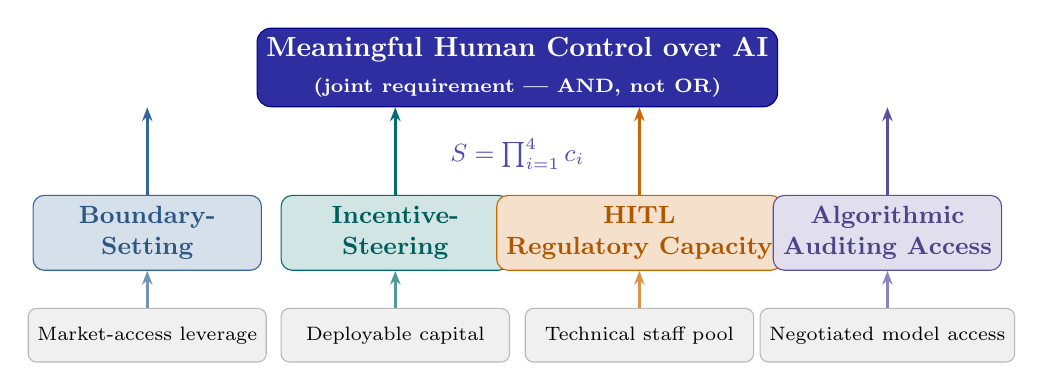
\begin{tikzpicture}[
  font=\normalsize,
  top/.style={rectangle,rounded corners=5pt,draw=darkblue,fill=darkblue!82,
              text=white,minimum width=6.4cm,minimum height=0.85cm,
              align=center,font=\normalsize\bfseries},
  p1/.style={rectangle,rounded corners=4pt,draw=steelblue,fill=steelblue!20,
             text=steelblue!85!black,minimum width=2.9cm,minimum height=0.95cm,
             align=center,font=\small\bfseries},
  p2/.style={rectangle,rounded corners=4pt,draw=tealcolor,fill=tealcolor!18,
             text=tealcolor!85!black,minimum width=2.9cm,minimum height=0.95cm,
             align=center,font=\small\bfseries},
  p3/.style={rectangle,rounded corners=4pt,draw=ambercolor,fill=ambercolor!20,
             text=ambercolor!85!black,minimum width=2.9cm,minimum height=0.95cm,
             align=center,font=\small\bfseries},
  p4/.style={rectangle,rounded corners=4pt,draw=slateblue,fill=slateblue!18,
             text=slateblue!85!black,minimum width=2.9cm,minimum height=0.95cm,
             align=center,font=\small\bfseries},
  res/.style={rectangle,rounded corners=3pt,draw=gray!55,fill=gray!12,
              minimum width=2.9cm,minimum height=0.68cm,align=center,
              font=\scriptsize},
  ar/.style={-{Stealth[length=5pt]},very thick},
  gate/.style={font=\small\bfseries,darkblue!70}
]
\node[top] (top) at (0,2.1) {Meaningful Human Control over AI\\[1pt]\scriptsize (joint requirement --- AND, not OR)};
\node[p1] (b1) at (-4.7,0.0) {Boundary-\\Setting};
\node[p2] (b2) at (-1.55,0.0) {Incentive-\\Steering};
\node[p3] (b3) at (1.55,0.0)  {HITL\\Regulatory Capacity};
\node[p4] (b4) at (4.7,0.0)   {Algorithmic\\Auditing Access};
\node[res] (r1) at (-4.7,-1.3) {Market-access leverage};
\node[res] (r2) at (-1.55,-1.3){Deployable capital};
\node[res] (r3) at (1.55,-1.3) {Technical staff pool};
\node[res] (r4) at (4.7,-1.3)  {Negotiated model access};
\draw[ar,steelblue] (b1) -- (top.south -| b1);
\draw[ar,tealcolor] (b2) -- (top.south -| b2);
\draw[ar,ambercolor] (b3) -- (top.south -| b3);
\draw[ar,slateblue] (b4) -- (top.south -| b4);
\draw[ar,steelblue!70] (r1) -- (b1);
\draw[ar,tealcolor!70] (r2) -- (b2);
\draw[ar,ambercolor!70] (r3) -- (b3);
\draw[ar,slateblue!70] (r4) -- (b4);
\node[gate] at (0,1.0) {$S=\prod_{i=1}^{4}c_i$};
\end{tikzpicture}%
}
\caption{The four-pillar framework. Each pillar rests on a distinct resource base (bottom row) and jointly feeds a single governance outcome (top). The product aggregation $S=\prod c_i$, formalized in Section~\ref{sec:case}.A, reflects that a missing pillar is not compensated by strength in the other three.}
\label{fig:pillars}
\end{figure}

\subsection{\textcolor{steelblue}{Boundary-Setting}}

Boundary-setting is what lets a government forbid a specific deployed behavior and make the prohibition stick against whoever operates the system. Writing the prohibition into statute is only the first step. The theoretical requirement is straightforward. A limit that cannot be enforced works only as a request. Enforcement requires legal authority over the entity operating the system. That is trivial when the operator is domiciled inside the regulator's jurisdiction and close to impossible when it is not.

This is where boundary-setting capacity concentrates sharply. The EU AI Act can compel compliance from any firm selling into the EU single market regardless of where that firm is headquartered, because market access itself is the enforcement lever~\cite{euaiact2024}.
A government without a market of comparable size has no equivalent lever: a firm that ignores its AI rules loses access to a market it may not have prioritized in the first place. Pakistan's IT and IT-enabled-services export sector, valued at a record approximately \$4.6 billion annually~\cite{sbp2026itexports},
is not large enough to make compliance with a Pakistan-specific AI rule a commercial priority for a frontier lab headquartered in California or Beijing --- and Pakistan's whole economy is roughly one-fiftieth the size of the EU's, a gap we derive from the two economies' GDP; no single source states it. Boundary-setting without market leverage is, in practice, advisory.

A second, less obvious resource requirement sits underneath boundary-setting: the ability to detect a violation in the first place. A prohibition a regulator cannot monitor is unenforceable even where market leverage exists, because enforcement presupposes evidence. Monitoring a deployed AI system at scale requires either direct API-level telemetry access, which vendors control, or independent technical means of probing system behavior in production --- both of which circle back to the data-access and technical-personnel constraints discussed under the remaining three pillars. Boundary-setting, in other words, is never purely a legal capacity; it is a legal capacity riding on top of a detection capacity that the framework treats as shared infrastructure across all four pillars.

\subsection{\textcolor{tealcolor}{Incentive-Steering}}

Incentive-steering is the capacity to pull AI development toward applications a society wants --- public-health diagnostics, agricultural forecasting, language tools for under-resourced languages --- instead of only writing rules against the uses it fears. This pillar is frequently absent from governance discussions entirely, which is itself a symptom of the capacity gap at issue. Restriction is cheap to legislate, while steering requires money.

Incentive-steering requires capital deployed at a scale that moves a market, and that capital exists almost exclusively inside the three major powers. The United States' CHIPS and Science Act directed tens of billions of dollars toward domestic semiconductor and AI-adjacent capacity~\cite{chipsact2022}.
China's state-directed AI industrial policy operates at a comparable or larger scale through a different mechanism, discussed in Section~\ref{sec:background}.C. The EU's funding instruments for AI research and deployment, while smaller than either, still dwarf what a mid-sized economy can allocate~\cite{eccommission2024aiinnovation}.
A government that cannot move capital at this scale cannot steer a market; it can only hope the market steers itself toward applications that happen to be useful locally, and that hope is frequently disappointed, because frontier labs optimize for the markets that fund them.

Compute is a second, distinct resource constraint on incentive-steering, separate from capital itself. A government that wants to seed domestic applications built on open-weight models, so as not to depend entirely on API access to foreign-hosted frontier systems, needs sovereign compute capacity to fine-tune and serve those models reliably~\cite{huang2026fivelayers}.
Capital without compute buys dependence on the same three jurisdictions already identified as dominant; a funding line that cannot also buy or build local compute access steers nothing, because the underlying infrastructure the funded projects run on remains rented from elsewhere.

NVIDIA's own account of where AI value accrues makes the same point from the supply side. Its chief executive has described the AI ecosystem as a five-layer stack of energy, chips, infrastructure, models, and applications, each layer reinforcing the ones above it~\cite{huang2026fivelayers}.
A government without incentive-steering capacity can, at best, participate at the top layer, building applications on infrastructure, chips, and energy supplied entirely by others; it has no purchase on the three layers beneath, which is where the resource-concentration argument places the United States, the European Union, and China. The scale at which capital moves through that stack has grown more than thirtyfold in about six years: NVIDIA's market capitalization stood near \$144 billion at the start of 2020 and reached \$5.5 trillion in mid-2026~\cite{nvidia2026marketcap},
a single firm's valuation increase alone exceeding ten times Pakistan's national GDP. A funding line calibrated to a national budget cannot move a market calibrated to numbers like these; it was never going to.

\subsection{\textcolor{ambercolor}{Human-in-the-Loop (HITL) Regulatory Capacity}}

HITL regulatory capacity is the existence of institutions staffed with people who understand how modern AI systems fail, and who can intervene at the speed of deployment cycles, a speed legislative cycles cannot match. The theoretical requirement here is specific and often underestimated. A regulator who cannot read a model's evaluation report, or who takes eighteen months to review a system update that ships every six weeks, is not exercising oversight --- it is rubber-stamping with a delay.

This pillar is bottlenecked by technical personnel, and technical personnel capable of evaluating frontier-scale systems are concentrated in the same three jurisdictions that train the systems. The EU AI Office employs more than 140 staff, over 40 of them in its AI safety unit, most with technical backgrounds~\cite{euaioffice2026staffing}.
NIST's AI Risk Management Framework work similarly draws on a dense US domestic pool of machine-learning researchers~\cite{nist2023airmf}.
By the AI Index's institutional-affiliation measures, AI research talent is concentrated overwhelmingly in these three jurisdictions~\cite{stanfordhai2026index}.
A finance ministry can create a regulatory body on paper in a week. It cannot create the pool of people who can staff it in a week, or, in most cases, in a decade.

HITL regulatory capacity also depends on data access in a way that is easy to overlook. A regulator cannot evaluate whether a deployed model behaves safely on a population it was never tested against without access to representative local data for that population. A model evaluated exclusively on English-language, US- or EU-sourced benchmark data may behave differently on Urdu-language queries or Pakistan-specific use cases, and no amount of regulatory staffing substitutes for the local evaluation datasets needed to test for that gap~\cite{stanfordhai2026index}.
Building and maintaining such datasets is itself a resource-intensive undertaking that again favors jurisdictions with existing data-infrastructure investment.

\subsection{\textcolor{slateblue}{Algorithmic Auditing and Self-Monitoring Access}}

Algorithmic auditing access means having real standing to open up a model someone else trained (its data provenance, its weights, its behavior under adversarial probing) without taking the vendor's self-reported documentation on faith. This is the pillar most absent from public AI-governance discourse, and the one we treat as the hardest to acquire externally, because it depends on access the vendor controls.

The risk this pillar exists to guard against has a documented historical precedent outside AI entirely. In 1904, a horse named Hans became famous across Germany for apparently solving arithmetic by tapping its hoof, and an official commission of veterinarians, trainers, and scientists examined the horse, found no evidence of deliberate fraud, and concluded the animal was genuinely performing the calculations. A further investigation by psychologist Oskar Pfungst later established the opposite: the horse had no arithmetic ability at all, and was instead reading involuntary, unconscious postural cues from its questioner, stopping exactly when the asker's body language signaled the correct tap count had been reached --- and failing completely once the questioner's cues were hidden from the horse's view~\cite{pfungst1911cleverhans}.
The commission's error was not carelessness; it was testing the horse under conditions that left the actual causal mechanism invisible to the test. A government evaluating a deployed AI system through a vendor-curated demonstration is in exactly the commission's position relative to the horse, not Pfungst's: it can observe the output, but not the mechanism producing it, and a system's apparent capability can be a property of infrastructure and scaffolding the evaluator never sees, rather than of the system being evaluated. Algorithmic auditing access is the institutional equivalent of being allowed to run Pfungst's follow-up test instead of only watching the horse perform.

The normal path to audit access runs through a negotiated agreement: a regulator inside the vendor's home jurisdiction requests structured access under statutory authority, and the vendor complies because refusal carries a market-access penalty under Section~\ref{sec:framework}.A's boundary-setting lever. The conflict path arises when the requesting government has no such lever: the vendor can offer a sandboxed, limited-scope demonstration instead of genuine model access.
The fallback for a government in that position is to rely on a mutual-recognition arrangement with a major-power regulator that did obtain genuine access, or to rely entirely on the vendor's self-published model card --- which is, definitionally, not an independent audit. Pakistan's National AI Policy does commit, in general terms, to impact assessments of high-impact systems and to a framework for third-party auditing of AI decision-making~\cite{pakistan2025nationalaipolicy}, but it contains no mechanism by which such an audit could be compelled from a foreign-hosted model provider.
That is not a drafting oversight; no comparably sized non-major economy currently has the leverage to negotiate the normal path, and the policy's silence on enforcement against foreign providers reflects that fact; it is not a gap its authors could simply have written around.

\subsection{\textcolor{darkblue}{Pillar Interdependence: Why the Four Do Not Substitute for One Another}}

A natural objection to treating these four pillars as separate is that strength in one could compensate for weakness in another --- that, for instance, enough incentive-steering capital could eventually buy the technical staff needed for HITL regulatory capacity, collapsing four pillars into one underlying resource: money. The objection has some force but ultimately fails, for a specific reason.

Capital converts into technical staff only on a multi-year timescale, because the relevant expertise does not exist as a purchasable commodity at the scale most governments would need. It belongs to people who can read a frontier model's training run, evaluate its failure modes, and know what a believable audit even looks like. A government can fund scholarships and fellowships; it cannot buy ten years of accumulated institutional experience inside a research and industry ecosystem that does not exist locally. Boundary-setting shows the same resistance to substitution from a different angle. No amount of domestic regulatory sophistication substitutes for market size, because enforcement against a foreign vendor runs through commercial leverage, which legal drafting skill cannot replace. Algorithmic auditing access resists substitution most starkly of the four, since it depends on a decision the vendor controls rather than a resource the regulating government can simply accumulate on its own schedule.

This interdependence argument is the qualitative version of the formal weakest-link aggregation developed in Section~\ref{sec:case}.A. It is presented here, ahead of the formal treatment, because the underlying intuition, that the four capacities complement one another and cannot stand in for each other, is doing real argumentative work on its own, independent of whether a reader accepts the specific mathematical model that follows.

\subsection{\textcolor{darkblue}{Toward New Law and Policy: Three Concrete Mechanisms}}

Diagnosing a capacity gap is not the same as specifying what should change in law and policy to close it. This subsection names three concrete mechanisms, each already proposed or precedented somewhere, and what adopting each would require and from whom.

\textbf{A compute-governance or licensing regime for frontier training runs.} The most developed version of this proposal combines domestic pre-approval regulation of training runs above a compute threshold with an international coordinating body, explicitly modeled on the International Atomic Energy Agency, to harmonize and monitor domestic regimes across jurisdictions, paired with a chip-export condition modeled on the Nuclear Non-Proliferation Treaty~\cite{belfield2025institutions}. A related, narrower proposal would require large compute providers (the cloud and data-center operators frontier labs run on) to implement know-your-customer obligations analogous to banking, so that a concerning training run becomes visible, and interruptible, before it completes~\cite{egan2023kyc}. A third model borrows directly from pharmaceutical and aviation regulation: no frontier-scale system may be trained or marketed without prior regulator approval based on submitted safety evidence, mirroring how a new drug cannot be sold without a trial record a regulator has reviewed~\cite{salvador2024certified}. None of these three currently has the force of law anywhere. Adopting any of them requires the three jurisdictions that hold the compute, capital, and chip-export leverage described in Section~\ref{sec:framework}.A--B to accept an external or shared oversight body with real standing over decisions each currently makes unilaterally, the kind of concession the framework predicts no major power has an unprompted incentive to make. The mechanism is specified; what is missing is the willingness to pay the political cost of adopting it.

\textbf{A binding technology-transfer or capacity-building obligation attached to a major-power regulatory regime.} This is the sharpest gap our review identified. The EU AI Act regulates third-country vendors selling into the EU extraterritorially, but contains no reciprocal obligation to build regulatory or technical capacity in the third countries whose markets those vendors also serve --- the Act's third-country provisions are a compliance burden on vendors, not a capacity transfer to governments~\cite{euaiact2024}. A real precedent for this kind of obligation exists in an adjacent domain: the Paris Agreement's Article 10, building on the UNFCCC's earlier technology-transfer commitment, requires support for developing-country parties and makes the standing UNFCCC Technology Mechanism serve the Agreement~\cite{unfccc2015parisart10}. The precedent has its own weakness. Whether delivery has matched the commitment is disputed, and nothing in the article compels it. An AI-governance equivalent would not automatically avoid that same enforcement gap. It would, however, give non-major economies a textual obligation to invoke and negotiate against, which is strictly more leverage than current AI-governance instruments offer them: none at all.

\textbf{A coalition-extended, mandatory, cross-border algorithmic audit right.} Two real instruments currently point in this direction without yet reaching it. The Algorithmic Accountability Act, introduced repeatedly in the US Congress, would mandate impact assessments and a new enforcement bureau, but it applies only domestically, with no extraterritorial reach for a government outside the United States~\cite{wyden2023algorithmic}. The EU AI Act's Notified Body conformity-assessment mechanism is the clearest enacted example of mandatory, legally binding third-party algorithmic audit with extraterritorial force~\cite{euaiact2024}, although its application to high-risk systems has been deferred to December 2027 and August 2028~\cite{euaiomnibus2026}; it exists to protect the EU single market, not to extend audit standing to a government that has no equivalent statute of its own. For a non-major economy, drafting a wholly new audit instrument alone is not a realistic near-term path, because such an instrument lacks enforcement teeth without market leverage (Section~\ref{sec:framework}.A). The likelier route is to negotiate a coalition-based extension of an existing mechanism such as the EU's Notified Body system. The research agenda in Section~\ref{sec:conclusion} ranks this coalition logic second, after audit-access mechanisms themselves.

These three mechanisms are not offered as a menu a single government can adopt unilaterally; each requires either a concession from a major power or a coalition a non-major economy cannot build alone. That constraint is the four-pillar finding again, stated as legislation. Where every major power declines, the fallback for a non-major economy is the deployer-side route of Section~\ref{sec:case}.D, which needs no concession from anyone.

\section{\textcolor{darkblue}{\hacof: From Governance Capacity to Continuous Operational Oversight}}
\label{sec:hacof}

Section~\ref{sec:framework} treats human control as a property of states, and Section~\ref{sec:case} tests that framing on Pakistan. The framing leaves one question untouched. Suppose a government does hold all four pillars. What, physically, stops a deployed AI agent from doing the thing the law forbids? This section proposes \hacof{} (Human-Centric AI Governance and Continuous Oversight Framework), a deployment-level reference model that answers that question in enough detail to be built and tested, and then shows which of its parts a weak regulator can require of deployers without building them itself. In short, the four pillars are what a state needs in order to require and verify \hacof-style controls; they are not what it needs in order to operate them.

\subsection{\textcolor{steelblue}{Why Capacity Needs an Operational Layer}}
\label{sec:hacof-a}

Take a firm whose written policy forbids its customer-service agent from disclosing client records, while the same agent holds read access to the whole client database, an outbound email tool, and permission to attach files. The policy exists. Nothing in the deployment enforces it. Whether the records stay inside depends on the model honoring an instruction --- the very property that indirect prompt injection is built to defeat~\cite{greshake2023injection}.
% CLAIM: Indirect prompt injection can cause LLM-integrated applications to deviate from intended behavior (e.g., exfiltrate data / act against the user).
An agent told never to run destructive commands but handed an unrestricted shell is the same case in a different costume, and its safety depends entirely on how reliably the model follows instructions. OWASP's risk catalog names the general condition excessive agency: a model-driven component granted more functionality, permission, or autonomy than its task requires~\cite{owasp2025llm}.
% CLAIM: OWASP Top 10 for LLM Applications (2025) lists "Excessive Agency" — excessive functionality, permissions, or autonomy granted to an LLM-based system — as a risk.

The four pillars decide whether a state can write a rule and check that it is obeyed, but they say nothing about whether the rule ever reaches the point at which an agent acts. Closing that distance involves five separate problems, and Table~\ref{tab:problems} traces each to the parts of \hacof{} that address it:
\begin{enumerate}
  \item \textit{Translation} --- legal and institutional requirements must become rules a machine can evaluate;
  \item \textit{Continuity} --- agents act around the clock, faster than a person can review action by action;
  \item \textit{Prevention and containment} --- a prohibited action should be stopped before it executes and, when that fails, contained quickly;
  \item \textit{Accountability} --- each decision, violation, and intervention must leave evidence an outside party can check;
  \item \textit{Second-order risk} --- whatever does the supervising can itself err, overreach, or be compromised.
\end{enumerate}
The five interact, so solving one in isolation buys little. Monitoring without enforcement records an incident it cannot stop, enforcement without independent review restricts arbitrarily, and a human overseer who lacks either the evidence to judge or a working control to stop the system cannot in practice intervene.

\begin{table}[!t]
\caption{The Five Problems and the \hacof{} Components That Address Them}
\label{tab:problems}
\centering
\footnotesize
\setlength{\tabcolsep}{3pt}
\begin{tabular}{>{\raggedright\arraybackslash}p{1.9cm}>{\raggedright\arraybackslash}p{3.6cm}>{\raggedright\arraybackslash}p{1.6cm}}
\toprule
\rowcolor{darkblue!15}
\textbf{Problem} & \textbf{Addressed by} & \textbf{Where} \\
\midrule
Translation & Layer 1 and 2: clause-traced authorization profiles; four boundary types & V.D \\
\rowcolor{darkblue!5}
Continuity & real-time monitoring; per-agent baselines; supervisory agents & V.E, V.F \\
Prevention and containment & in-path guardrails; Prevent--Contain--Recover lifecycle; containment conditions & V.D, V.G \\
\rowcolor{darkblue!5}
Accountability & audit plane; human roles; appeal path; regulator-facing records & V.H \\
Second-order risk & supervisor diversity; governance of the governors; privacy limits & V.E, V.I, V.J \\
\bottomrule
\end{tabular}
\end{table}

\hacof{} brings together six working parts, each developed below. Its AI policies bind because they rest on law, and its technical safety controls sit outside the model; Section~\ref{sec:hacof}.D covers both. Independent supervisory agents follow in Section~\ref{sec:hacof}.E and real-time behavioral monitoring in Section~\ref{sec:hacof}.F. Containment can act automatically, but only under the conditions stated in Section~\ref{sec:hacof}.G. Section~\ref{sec:hacof}.H sets out the human governance under which a named person answers for each consequential intervention. The limits an agent works within come from four sources, namely law, ethics, the deployer's operations, and the technical configuration, and Section~\ref{sec:hacof}.D treats each separately. Within those limits, supervisors keep watch over what the agents do, flag breaches of policy, notice dangers that no rule yet names, and set off responses scaled to the danger.

The governing structure is a hierarchy, and its order matters. Foundational human rights, together with whatever law applies, set the highest-level constraints. Institutional policies translate those constraints into rules specific enough to enforce. Technical guardrails stop unauthorized actions before they happen. Independent supervisory agents then watch for compliance across the whole AI lifecycle, from authorization through execution to review. A high-risk violation backed by clear evidence can trigger immediate technical containment; a decision that is ambiguous or consequential goes to an authorized human reviewer instead. Experimentation, research, and ordinary automation continue under \hacof{}, inside limits that people set and can inspect.

\subsection{\textcolor{tealcolor}{Three Distinctions That Bound the Claim}}
\label{sec:hacof-b}

Three distinctions recur through the rest of this section, and each one also limits what \hacof{} can be said to contribute.

\textbf{Safety versus policing.} Safety mechanisms act \textit{within} a single system. Constitutional training shapes a model's dispositions against written principles~\cite{bai2022constitutional},
% CLAIM: Constitutional AI trains a model using a written set of principles (a "constitution") with AI feedback.
and guardrail classifiers screen what goes into and comes out of that one model~\cite{inan2023llamaguard,sharma2025constitutionalclassifiers}.
% CLAIM: Llama Guard and Constitutional Classifiers are classifiers that screen LLM inputs and/or outputs for a single model deployment.
Policing acts \textit{across} systems: something outside the governed agents checks whether their combined activity complies with rules that bind all of them. A well-aligned model can still be handed excessive privileges, and a well-run monitor cannot make a badly aligned model safe, so the two complement each other. \hacof{} claims neither half. What it adds, as the end of this subsection sets out, is a legal chain of authority that runs from statute down to specific enforcement points and extends to the supervisors themselves.

\textbf{Detection versus prevention.} A monitor can recognize suspicious activity. Only a component sitting on the execution path, with the authority to deny an action before it completes, can prevent it. A monitor that watches a copy of the traffic --- \textit{out-of-path} --- can raise an alarm, revoke a credential after the fact, or isolate a workload, but it cannot guarantee that the first harmful action never happens. An \textit{in-path} enforcement point can, for exactly the actions that are routed through it and for no others. The engineering precedent is runtime assurance in the Simplex style, where a complex, unverified controller runs alongside a simple, high-assurance controller, and decision logic switches control to the high-assurance controller when the system nears the edge of its safe envelope~\cite{sha2001simplex}.
% CLAIM: Simplex: a complex unverified controller runs alongside a simple high-assurance controller; decision logic switches control to the latter near the edge of the safe envelope.
\hacof{} applies the same pattern to agents: the agent is the complex controller, the in-path gateway is the decision module, and the safe fallback is denial plus escalation to a human. Tables~\ref{tab:supervisors} and~\ref{tab:enforcement} and Fig.~\ref{fig:lifecycle} mark which capabilities and responses depend on an in-path point, and Section~\ref{sec:hacof}.K bounds what prevention can achieve when some actions bypass such points.

\textbf{Oversight versus surveillance.} \hacof{} monitors what AI systems do: tool calls, data access, credentials, delegation, transactions. It does not license unlimited observation of the people who use those systems or appear in their data. Privacy law, due process, and independent review bind the supervisory machinery exactly as they bind any other data processor, a point Section~\ref{sec:hacof}.J develops.

The novelty claim is correspondingly modest. AI monitoring AI is established~\cite{greenblatt2024aicontrol,shavit2023agentic,gosmar2025sentinel};
% CLAIM: Prior work already proposes automated/AI monitoring of AI systems (trusted monitoring; Shavit 4.5 automatic monitoring; sentinel agents).
layered translation of governance standards into runtime controls has been sketched~\cite{koch2026layered};
% CLAIM: Koch maps governance standards to layered controls incl. runtime mediation.
graduated enforcement for agents has been prototyped~\cite{gaurav2025gaas,wang2025mi9};
% CLAIM: GaaS and MI9 implement graduated enforcement/containment for agents.
explicit trust boundaries with policy decision and policy enforcement points are the core of zero-trust security architecture~\cite{nist2020zerotrust};
% CLAIM: NIST SP 800-207: no implicit trust; PDP/PEP grant access per session.
and the NIST AI Risk Management Framework already organizes organizational risk work into its Govern, Map, Measure, and Manage functions~\cite{nist2023airmf}.
% CLAIM: NIST AI RMF 1.0 is organized into four core functions: Govern, Map, Measure, and Manage.
The AI RMF is process guidance for organizations, voluntary in the United States; \hacof{} is a runtime enforcement architecture that could implement parts of what Measure and Manage ask for, alongside the framework. \hacof{} is therefore offered as a reference model for policy makers, one that assembles these established techniques under legal authority, and not as a new technical architecture. What it adds is narrower: a legitimacy chain from statute to enforcement point, in which no automated component may originate a rule; a second-order governance regime and binding privacy limits for the supervisors themselves; a supervisor-diversity requirement grounded in evidence about correlated model errors; and the mapping to state capacity in Section~\ref{sec:hacof}.M.

Table~\ref{tab:priorwork} sets these neighbors side by side. Read by row, it shows how much of \hacof{} already exists elsewhere; read by column, it shows where the gaps are. Several prior works, Shavit et al.\ and Chan et al.\ above all, raise the monitor's own reliability, its privacy cost, and the risk of monitors trained like the agents they watch as open concerns. None turns them into design requirements. The last four columns, where no prior row reaches a full mark, are where the contribution should be judged.

\begin{table*}[!t]
\caption{\hacof{} Positioned Against Prior Frameworks and Instruments}
\label{tab:priorwork}
\centering
\footnotesize
\setlength{\tabcolsep}{3.5pt}
\begin{tabular}{>{\raggedright\arraybackslash}p{3.7cm}*{8}{>{\centering\arraybackslash}p{1.5cm}}}
\toprule
\rowcolor{darkblue!15}
\textbf{Framework} & \textbf{Authority traced to law} & \textbf{In-path enforcement} & \textbf{Specialized AI supervisors} & \textbf{Graduated containment} & \textbf{Governance of supervisors} & \textbf{Binding privacy limits on monitor} & \textbf{Supervisor diversity required} & \textbf{State-capacity analysis} \\
\midrule
\rowcolor{darkblue!5}Agentic-AI practices~\cite{shavit2023agentic} & -- & $\circ$ & $\circ$ & -- & $\circ$ & $\circ$ & $\circ$ & -- \\
AI control~\cite{greenblatt2024aicontrol} & -- & $\circ$ & $\circ$ & $\circ$ & $\circ$ & -- & -- & -- \\
\rowcolor{darkblue!5}Visibility into agents~\cite{chan2024visibility} & -- & $\circ$ & -- & -- & $\circ$ & $\circ$ & -- & -- \\
GuardAgent/ShieldAgent~\cite{xiang2025guardagent,chen2025shieldagent} & $\circ$ & \checkmark & $\circ$ & -- & -- & -- & -- & -- \\
\rowcolor{darkblue!5}AgentSpec~\cite{wang2026agentspec} & $\circ$ & \checkmark & -- & -- & -- & -- & -- & -- \\
Sentinel agents~\cite{gosmar2025sentinel} & -- & \checkmark & \checkmark & \checkmark & $\circ$ & $\circ$ & -- & -- \\
\rowcolor{darkblue!5}GaaS~\cite{gaurav2025gaas} & -- & \checkmark & -- & \checkmark & -- & -- & -- & -- \\
MI9~\cite{wang2025mi9} & -- & \checkmark & -- & \checkmark & -- & -- & -- & -- \\
\rowcolor{darkblue!5}Layered standards mapping~\cite{koch2026layered} & $\circ$ & $\circ$ & -- & $\circ$ & -- & -- & -- & -- \\
IMDA agentic framework~\cite{imda2026agentic} & $\circ$ & $\circ$ & $\circ$ & $\circ$ & -- & -- & -- & -- \\
\rowcolor{darkblue!5}NIST AI RMF~\cite{nist2023airmf} & $\circ$ & -- & -- & $\circ$ & -- & -- & -- & -- \\
EU AI Act~\cite{euaiact2024,euaiomnibus2026} & \checkmark & $\circ$ & -- & $\circ$ & -- & -- & -- & -- \\
\rowcolor{tealcolor!15}\textbf{\hacof{} (this work)} & \checkmark & \checkmark & \checkmark & \checkmark & \checkmark & \checkmark & \checkmark & \checkmark \\
\bottomrule
\multicolumn{9}{p{17.2cm}}{\scriptsize \checkmark\ = addressed as a design requirement; $\circ$ = partly addressed (e.g., one monitor rather than specialized roles, voluntary rather than legal authority, raised as a concern rather than a constraint); -- = not addressed as a design requirement in the cited source. Entries summarize the cited work's stated scope; they are not a quality ranking. \hacof{}'s entries describe its design, which has been tested only in simulation (Section~\ref{sec:eval}.D).}
\end{tabular}
\end{table*}

\subsection{\textcolor{ambercolor}{Aims, Foundational Principles, and Design Objectives}}
\label{sec:hacof-objectives}

\hacof{} has one aim stated in three parts: to make AI-related harm less likely to occur, less severe when it does occur, and shorter-lived once it has started, while keeping room for beneficial innovation and protecting human autonomy, privacy, accountability, and due process. Each part maps to a phase of the lifecycle in Section~\ref{sec:hacof}.G --- likelihood to prevention, severity to containment, duration to recovery.

No architecture can promise to stop every harmful action. Detectors miss things, enforcement points can be bypassed, and supervisors can be wrong, as Sections~\ref{sec:hacof}.K and~\ref{sec:limits} make explicit. \hacof{} is therefore built on four foundational principles, each of which starts by assuming failure.

\begin{mdframed}[linecolor=tealcolor, linewidth=1.2pt, backgroundcolor=tealcolor!5,
  innerleftmargin=8pt, innerrightmargin=8pt, innertopmargin=6pt, innerbottommargin=6pt,
  roundcorner=4pt]
\noindent\textbf{\textcolor{tealcolor}{Foundational Principles ---}}
\begin{itemize}
  \item \textit{Defense in depth:} every risk is met by more than one control, of more than one kind (a guardrail, a supervisor, and a person), so one failure is not a breach.
  \item \textit{Independent verification:} no control certifies itself; decisions are checked by a component built differently and holding different credentials.
  \item \textit{Resilience:} when any part fails, the system degrades toward restriction, never toward openness, and service can be restored without losing the record.
  \item \textit{Continuous improvement:} every incident and every false positive feeds an approved, regression-tested change to rules or baselines.
\end{itemize}
\end{mdframed}

To be useful, a reference model must be testable, so \hacof{} commits to eight design objectives, each stated so that it can be checked and each tied to at least one metric of the evaluation protocol in Table~\ref{tab:metrics} (Section~\ref{sec:eval}). Table~\ref{tab:objectives} lists them. Thresholds are deliberately absent. The acceptable detection rate for a payments agent and for an internal summarization agent differ, and Section~\ref{sec:eval} requires the deployer to fix them per risk category before testing begins, not after the results are in.

\begin{table}[!t]
\caption{\hacof{} Design Objectives and Their Checks}
\label{tab:objectives}
\centering
\footnotesize
\setlength{\tabcolsep}{3pt}
\begin{tabular}{>{\raggedright\arraybackslash}p{1.75cm}>{\raggedright\arraybackslash}p{3.15cm}>{\raggedright\arraybackslash}p{2.25cm}}
\toprule
\rowcolor{darkblue!15}
\textbf{Objective} & \textbf{Checkable criterion} & \textbf{Metric (Table~\ref{tab:metrics})} \\
\midrule
O1 Authority hierarchy & every enforced rule resolves to a named legal or policy clause; no rule without one & audit completeness \\
\rowcolor{darkblue!5}
O2 Continuous monitoring & every governed action emits telemetry the monitoring plane receives & detection rate; time to detection \\
O3 Independent supervisors & diverse supervisors outperform the homogeneous ablation & detection rate (by ablation arm) \\
\rowcolor{darkblue!5}
O4 Prevent and contain & prohibited actions on gated paths are denied before execution; others contained & prevention effectiveness; time to containment; residual harm \\
O5 Accountability and appeal & any intervention can be explained, reviewed, and reversed by a person & audit completeness; review and appeal outcomes \\
\rowcolor{darkblue!5}
O6 Rights and legitimate use & lawful but unusual work proceeds; monitoring data stay within purpose & false-positive rate; privacy impact \\
O7 Measurability & every metric reported per risk category with uncertainty & all ten, per Section~\ref{sec:eval} \\
\rowcolor{darkblue!5}
O8 Continuous improvement & policy updates pass regression tests; no silent loosening & false-positive and detection rates across versions; recovery time \\
\bottomrule
\end{tabular}
\end{table}

Two of the eight carry most of the weight. O1 is what separates \hacof{} from a well-instrumented security stack. If a deny decision cannot be traced to a clause someone with authority wrote, the system is enforcing its own preferences. O6 keeps it from turning into a surveillance stack. The remaining six are conventional engineering objectives, stated here so that a failed pilot can be diagnosed objective by objective.

\subsection{\textcolor{slateblue}{Six Layers, Six Planes, and Four Boundary Types}}
\label{sec:hacof-arch}

Within this section, a \textit{layer} is a level of the governance hierarchy, defined by where authority comes from and which kind of control carries it, and a \textit{plane} is a part of the running deployment where machinery executes. The ``five-layer stack'' of Section~\ref{sec:framework}.B uses the word in its industry sense and is unrelated. \hacof{} has six of each. The six layers are: (L1) human authority and legal governance; (L2) machine-readable policy and permission architecture; (L3) preventive technical guardrails; (L4) independent supervisory agents; (L5) the continuous monitoring, containment, and enforcement lifecycle; and (L6) accountable human governance, audit, and continuous improvement. Layers 1--3 form the \textit{authority chain} that turns law into a technical restriction. Layers 4--6 watch, respond, and answer for what happens. Table~\ref{tab:layers} states the relation between the two views once.

\begin{table}[!t]
\caption{\hacof{} Layers (Governance View) and Planes (Deployment View)}
\label{tab:layers}
\centering
\footnotesize
\setlength{\tabcolsep}{3pt}
\begin{tabular}{>{\raggedright\arraybackslash}p{2.35cm}>{\raggedright\arraybackslash}p{2.5cm}>{\raggedright\arraybackslash}p{2.3cm}}
\toprule
\rowcolor{darkblue!15}
\textbf{Layer} & \textbf{Function} & \textbf{Runs in plane(s)} \\
\midrule
L1 Human authority \& legal governance & rights, law, risk classes, duties, remedies & none directly; encoded into the control plane \\
\rowcolor{darkblue!5}
L2 Policy \& permission architecture & authorization profiles; conflict order & control \\
L3 Preventive guardrails & eight enforcement mechanisms & enforcement (identities held in control) \\
\rowcolor{darkblue!5}
L4 Supervisory agents & Agents A--G & monitoring; A, D, E also feed enforcement gates \\
L5 Monitoring, containment \& enforcement lifecycle & baselines; nine-step loop; playbooks & monitoring, enforcement \\
\rowcolor{darkblue!5}
L6 Human governance, audit \& improvement & roles; appeals; audit; approved change & human governance, audit \\
--- (governed systems) & agents, models, tools & execution \\
\bottomrule
\end{tabular}
\end{table}

\textbf{Four boundary types.} The limits an agent works within come from four sources, which differ in who sets them and in how far a machine can check them. Table~\ref{tab:boundaries} summarizes the differences.

\begin{table}[!t]
\caption{The Four Boundary Types in \hacof}
\label{tab:boundaries}
\centering
\footnotesize
\setlength{\tabcolsep}{3pt}
\begin{tabular}{>{\raggedright\arraybackslash}p{1.45cm}>{\raggedright\arraybackslash}p{1.7cm}>{\raggedright\arraybackslash}p{2.1cm}>{\raggedright\arraybackslash}p{1.9cm}}
\toprule
\rowcolor{darkblue!15}
\textbf{Boundary} & \textbf{Set by} & \textbf{Machine-checkable?} & \textbf{Enforced as} \\
\midrule
Legal & legislature, regulator, courts & specific prohibitions yes; open standards (``reasonable'', ``proportionate'') no & profile rules with a clause pointer; open standards become review triggers \\
\rowcolor{darkblue!5}
Ethical & deployer's ethics body, professional codes, public consultation & only partly; most need contextual judgment & adopted policy rules where precise; otherwise human-review triggers \\
Operational & deployer (policy owner) & yes: purpose, scope, channels, hours, budgets & profile fields \\
\rowcolor{darkblue!5}
Technical & security and platform engineers & yes, by construction & permissions, sandboxes, rate limits, credentials \\
\bottomrule
\end{tabular}
\end{table}

\textit{Legal} boundaries are the outer limit and the only source of prohibitions with the force of law. Much of law is checkable only in part. ``Do not export customer records outside the jurisdiction'' compiles to a rule a gateway can evaluate; ``process data fairly'' does not. \hacof{} handles the second kind by routing the relevant class of action to a human reviewer; a classifier verdict never stands in for a legal finding.

\textit{Ethical} boundaries are the hardest to operationalize. Some ethical commitments are precise enough to write down (a hospital may decide that no agent drafts a diagnosis without a clinician's name attached), and once the deployer adopts them as policy, through the policy owner's ordinary approval, they are enforced like any other rule. Many are not that precise. Whether a particular persuasive message to a vulnerable customer crosses a line depends on context a gateway does not have, so those commitments enter \hacof{} as review triggers and as criteria human reviewers apply. We make no claim that ethics can be compiled; an architecture that claimed so would end up enforcing whichever approximation was easiest to code.

\textit{Operational} boundaries are the deployer's own business limits: this agent handles refunds and not loans; it may email customers and not journalists; it may run between these hours and spend this much compute. They are fully checkable and change most often.

\textit{Technical} boundaries are the mechanisms (permissions, sandboxes, rate limits, credentials) through which the other three are enforced. They are checkable by construction but carry no authority of their own. A technical setting that permits what a legal or operational boundary forbids is a configuration defect, and the gateway treats it as one.

When boundaries conflict, the order is legal, then ethical as adopted into policy, then operational, with technical settings bound to implement whichever of the three is strictest. Two conflicts deserve explicit handling. Where an ethical commitment is stricter than the law, as with data minimization beyond what statute requires, the stricter commitment applies, because policy may tighten law. Where an ethical preference would require breaking a legal duty, such as deleting records a regulator requires the deployer to keep, the legal duty wins, and the ethical aim is pursued within it, for instance by restricting who can read the retained records. Any conflict the ordering does not settle is escalated to the policy owner, and the action is held under the more restrictive reading until a person decides.

\textbf{Layer 1: human authority and legal governance.} Legislatures, regulators, and courts set the outer boundary. Layer~1 records nine kinds of content that the layers below depend on: the human rights the system must respect and the legal restrictions that protect them; prohibited applications and conduct; risk classifications; the respective duties of developers, deployers, operators, and service providers; independent audit and incident-reporting duties; authorization procedures for high-risk applications; penalties and remedies; and channels for complaints, appeals, and independent review. The ninth is a separation between principles that hold everywhere, such as respect for life and non-discrimination, and obligations that hold only in a given jurisdiction, such as a data-localization rule or a sector licensing condition. The EU AI Act has written several of these into law, including logging for high-risk systems, human oversight, deployer obligations, and serious-incident reporting~\cite{euaiact2024},
% CLAIM: EU AI Act contains logging/record-keeping (Art. 12), human oversight (Art. 14), deployer obligations (Art. 26), and serious-incident reporting (Art. 73) provisions.
although a 2026 amending regulation defers their application to high-risk systems until December 2027 or August 2028~\cite{euaiomnibus2026}.
% CLAIM: Regulation (EU) 2026/1744 moves application of Chapter III Sections 1-3 to 2 Dec 2027 (Annex III) / 2 Aug 2028 (Annex I).
Two rules govern how organizations translate law into internal policy. Policy may tighten the law but never loosen it. And no automated component may originate a prohibition. Every enforcement action further down traces to a human or legal source, never to a monitor's view that something ought to be forbidden. Enforcement authority in \hacof{} is borrowed from people and institutions with the legitimacy to grant it; the supervisory machinery holds none of its own.

\textbf{Cross-border deployments.} A deployment that serves users in several jurisdictions carries jurisdiction tags in each agent's profile, and an action touching more than one jurisdiction is evaluated against the union of applicable rules, so the strictest applies. Where two jurisdictions impose duties that cannot both be met (one requires a record to be disclosed, the other forbids its export), the action is held, the conflict goes to human counsel, and the deployment runs under the more restrictive reading until it is resolved, a fail-safe default in the classic sense~\cite{saltzer1975protection}.
% CLAIM: Saltzer and Schroeder list fail-safe defaults (base access decisions on permission rather than exclusion) among their design principles.
Evidence for a regulator in another jurisdiction is shared through the audit-plane interface of Section~\ref{sec:hacof}.H under whatever mutual-recognition arrangement exists (Section~\ref{sec:case}.D); interoperable profile formats across organizations remain an open problem (Section~\ref{sec:limits}).

\textbf{Layer 2: machine-readable policy and permission architecture.} Each agent receives an authorization profile that states its approved purpose and scope; the data it may read; the tools and services it may call; the actions it may take on its own; the actions that need human approval; its compute, rate, and time limits; its permitted communication channels; its permitted delegation; its logging duties; and the conditions under which its privileges are suspended. Table~\ref{tab:profile} works through a profile for an agent that reconciles a bank's accounts. Profiles are version-controlled and tested before deployment, and each rule points to the clause it implements. A rule with no traceable source is a defect, not a precaution. ISO/IEC 42001 and NIST's generative-AI profile can supply the management scaffolding around them~\cite{iso2023iso42001,nist2024genai}.
% CLAIM: ISO/IEC 42001:2023 specifies requirements for an AI management system in organizations; NIST AI 600-1 is a Generative AI Profile of the AI RMF.

\begin{table}[!t]
\caption{Worked Authorization Profile (Illustrative): Account-Reconciliation Agent}
\label{tab:profile}
\centering
\footnotesize
\setlength{\tabcolsep}{3pt}
\begin{tabular}{>{\raggedright\arraybackslash}p{1.5cm}>{\raggedright\arraybackslash}p{3.15cm}>{\raggedright\arraybackslash}p{2.5cm}}
\toprule
\rowcolor{darkblue!15}
\textbf{Field} & \textbf{Value} & \textbf{Traced to (hypothetical)} \\
\midrule
Purpose & reconcile ledger entries; report mismatches & internal policy FIN-RECON \S1 \\
\rowcolor{darkblue!5}
May read & general ledger; bank statements, current quarter & FIN-RECON \S2; data-protection purpose clause \\
May call & ledger API (read), report generator; payment interface (approval-gated) & FIN-RECON \S3; banking-regulator payment rule \\
\rowcolor{darkblue!5}
Autonomous & read; compare; draft report & FIN-RECON \S3 \\
Needs approval & export records; initiate or alter a transfer & banking-regulator payment rule; FIN-RECON \S4 \\
\rowcolor{darkblue!5}
Limits & read rate cap; business hours; compute budget & operational policy OPS-2 \\
Channels & internal report queue only; no email & data-localization clause \\
\rowcolor{darkblue!5}
Delegation & one sub-agent, read-only subset, depth 1 & FIN-RECON \S5 \\
Logging & every call, full metadata; retained per records rule & record-retention clause \\
\rowcolor{darkblue!5}
Suspend if & export attempt; access outside quarter; Agent C credential alert & FIN-RECON \S6 \\
\bottomrule
\end{tabular}
\end{table}

\textit{Delegation rule.} A sub-agent's profile is derived from its parent's and can only narrow it: every permission, data scope, tool, and limit in the child's profile must be a subset of the parent's, delegation depth is capped by the parent's profile, and the child cannot itself hold the right to delegate unless the parent explicitly passes on a narrower version of that right. The gateway enforces the subset relation when the child is created; a child profile that is not a subset is rejected and the parent's attempt is logged as an anomaly. Permissions therefore shrink monotonically down any delegation chain and never widen.

Conflicts between instructions resolve by a fixed order: law, then safety restrictions, then organizational policy, then the agent's profile, then operator instructions, then user instructions, and last, content arriving through tools or retrieved documents. The ordering resembles the instruction hierarchy of Wallace et al., which trains a model to give system messages priority over user messages and both over tool outputs~\cite{wallace2024hierarchy}.
% CLAIM: Wallace et al.'s instruction hierarchy trains LLMs to prioritize system-level instructions over user instructions and over lower-privileged inputs such as tool outputs.
The difference is where the ordering lives. A learned hierarchy is a disposition of the model and holds with some probability; \hacof's is enforced outside the model, so a lower-priority instruction cannot widen an agent's permissions, because the permissions are not stored anywhere that instruction can reach. When a profile itself turns out to contradict a higher rule, the higher rule wins, the action is denied, and the contradiction is queued for the policy owner to fix the profile.

\textbf{Layer 3: preventive technical guardrails.} An agent \textit{instructed} to be safe and an agent \textit{restricted} to be safe are different objects. The first is a forecast about model behavior. The second is a property of the environment, and it holds even when the forecast fails. Layer~3 supplies the second kind through eight mechanisms:
\begin{enumerate}
  \item \textit{Identity and authorization} --- every agent, tool, and task carries a verifiable identity, and every permission is scoped to it;
  \item \textit{Least privilege} --- each agent holds only the permissions its profile names~\cite{saltzer1975protection};
% CLAIM: Saltzer and Schroeder: least privilege — every program and user should operate using the least set of privileges necessary.
  \item \textit{Tool gateways} --- every tool call passes a gateway that checks it against the profile, which is complete mediation applied to agents~\cite{saltzer1975protection};
% CLAIM: Saltzer and Schroeder: complete mediation — every access to every object must be checked for authority.
  \item \textit{Data-loss prevention} --- outbound channels are inspected for personal and confidential data;
  \item \textit{Sandboxing} --- code an agent writes or runs executes in an isolated environment with no route to production systems;
  \item \textit{Transaction controls} --- high-impact actions such as moving funds, changing critical infrastructure, or altering security settings are held for approval;
  \item \textit{Resource limits} --- caps on call rate, quota, run time, and concurrency bound how much an agent can do before anyone notices;
  \item \textit{Revocable credentials} --- short-lived credentials that the enforcement plane can withdraw at once.
\end{enumerate}
This is zero-trust architecture applied to agents: no implicit trust by network location or prior session, and an explicit policy decision point consulted before access is granted, session by session~\cite{nist2020zerotrust}.
% CLAIM: Zero trust (NIST SP 800-207): no implicit trust based on network location; access granted per session via PDP/PEP.
For agents, \hacof{} tightens the session granularity of that model to the individual tool call. Classifier guards feed the gateway as one signal among several; they do not replace it. If the gateway cannot reach its policy decision point, it denies. If a denied action has a legitimate need behind it, the agent's operator files an approval request to the human governance plane; the control itself stays in place.

\textbf{Six planes and the end-to-end flow.} Fig.~\ref{fig:hacof} shows the deployment view as a seven-stage flow. Human authorities and law (L1) yield approved policies, risk classes, and the enforcement configuration, held in the \textit{control plane} (L2). Those become identity, authorization, and preventive controls in the \textit{enforcement plane} (L3), which sits in front of the agents, models, tools, and outside interactions of the \textit{execution plane}. Independent monitoring and the supervisory agents (L4) run in the \textit{monitoring plane}. Enforcement, containment, and evidence preservation (L5) act through the enforcement plane and are sealed in the \textit{audit plane}. Human review, independent audit, corrective action, and policy improvement (L6) happen in the \textit{human governance plane}, which alone can send approved changes back to the control plane. The figure is drawn top to bottom, but monitoring and enforcement run continuously across the whole stack: critical operations are evaluated before they execute, and everything, including actions that passed the pre-execution check, is still monitored afterward, because prevention will miss things.

Separation is the point. A compromised workload in the execution plane holds no credential that writes to the control or audit plane, so it cannot rewrite its own profile, erase its trail, or switch off the gateway in front of it --- separation of privilege applied across the deployment~\cite{saltzer1975protection}.
% CLAIM: Saltzer and Schroeder's separation of privilege principle: a mechanism requiring two keys is more robust than one requiring a single key.

\begin{figure}[H]
\centering
\resizebox{\columnwidth}{!}{%
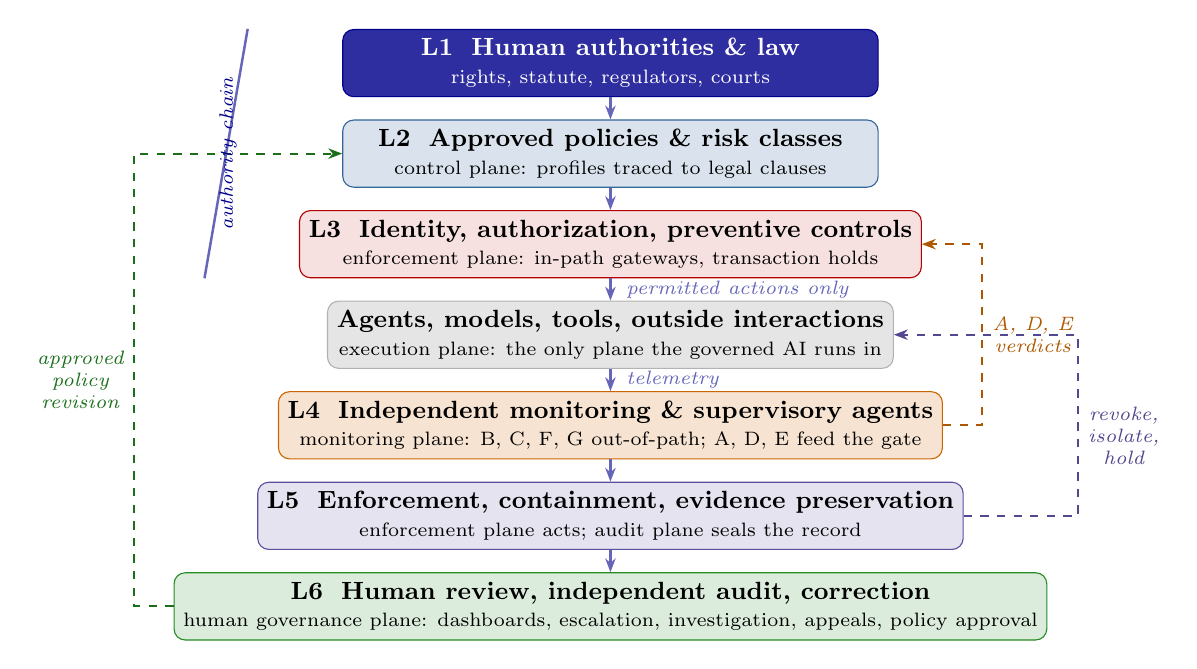
\begin{tikzpicture}[
  font=\normalsize,
  lay/.style={rectangle,rounded corners=4pt,draw=darkblue,fill=darkblue!82,
              text=white,minimum width=6.8cm,minimum height=0.8cm,
              align=center,font=\small\bfseries},
  pl/.style={rectangle,rounded corners=4pt,minimum width=6.8cm,
             minimum height=0.8cm,align=center,font=\small},
  ar/.style={-{Stealth[length=5pt]},thick,darkblue!60},
  side/.style={-{Stealth[length=5pt]},thick,dashed},
  tag/.style={font=\scriptsize\itshape,align=center}
]
\node[lay] (l1) at (0,0) {L1 \;Human authorities \& law\\[-1pt]
  \scriptsize\mdseries rights, statute, regulators, courts};
\node[pl,draw=steelblue,fill=steelblue!18] (cp) at (0,-1.15)
  {\textbf{L2 \;Approved policies \& risk classes}\\[-1pt]
  \scriptsize control plane: profiles traced to legal clauses};
\node[pl,draw=deepred,fill=deepred!12] (ep) at (0,-2.30)
  {\textbf{L3 \;Identity, authorization, preventive controls}\\[-1pt]
  \scriptsize enforcement plane: in-path gateways, transaction holds};
\node[pl,draw=gray!60,fill=gray!20] (xp) at (0,-3.45)
  {\textbf{Agents, models, tools, outside interactions}\\[-1pt]
  \scriptsize execution plane: the only plane the governed AI runs in};
\node[pl,draw=ambercolor,fill=ambercolor!18] (mp) at (0,-4.60)
  {\textbf{L4 \;Independent monitoring \& supervisory agents}\\[-1pt]
  \scriptsize monitoring plane: B, C, F, G out-of-path; A, D, E feed the gate};
\node[pl,draw=slateblue,fill=slateblue!16] (cn) at (0,-5.75)
  {\textbf{L5 \;Enforcement, containment, evidence preservation}\\[-1pt]
  \scriptsize enforcement plane acts; audit plane seals the record};
\node[pl,draw=midgreen,fill=midgreen!16] (hp) at (0,-6.90)
  {\textbf{L6 \;Human review, independent audit, correction}\\[-1pt]
  \scriptsize human governance plane: dashboards, escalation, investigation, appeals, policy approval};
\draw[ar] (l1) -- (cp);
\draw[ar] (cp) -- (ep);
\draw[ar] (ep) -- node[right,tag,xshift=2pt]{permitted actions only} (xp);
\draw[ar] (xp) -- node[right,tag,xshift=2pt]{telemetry} (mp);
\draw[ar] (mp) -- (cn);
\draw[ar] (cn) -- (hp);
% in-path verdicts of A, D, E reach the gate
\draw[side,ambercolor!85!black] (mp.east) -- ++(0.5,0) |- node[pos=0.25,right,tag]{A, D, E\\verdicts} (ep.east);
% containment acts back on running agents
\draw[side,slateblue!90!black] (cn.east) -- ++(1.45,0) |- node[pos=0.22,right,tag]{revoke,\\isolate,\\hold} (xp.east);
% feedback: human review revises policy
\draw[side,midgreen!80!black] (hp.west) -- ++(-0.5,0) |- node[pos=0.25,left,tag]{approved\\policy\\revision} (cp.west);
% authority-chain bracket
\draw[darkblue!60,line width=0.9pt] ([xshift=-1.2cm]l1.north west) -- ([xshift=-1.2cm]ep.south west);
\node[tag,rotate=90,darkblue] at ([xshift=-1.45cm]cp.west) {authority chain};
\end{tikzpicture}%
}
\caption{\hacof{} end-to-end flow across the six layers (L1--L6) and six planes. Layers 1--3 (left bracket) carry authority from law to an in-path enforcement point in front of the execution plane. The monitoring plane is out-of-path except where a supervisor's verdict is wired into the gate (Agents A, D, E in Table~\ref{tab:supervisors}; right, inner dashed line). Containment acts back on running workloads (right, outer dashed line). Only human review can send approved policy revisions to the control plane (left, dashed); no automated component edits policy directly. Monitoring and enforcement run continuously across the stack.}
\label{fig:hacof}
\end{figure}

\subsection{\textcolor{darkblue}{Supervisory Agents: \hacof's Central Operational Component}}
\label{sec:hacof-supervisors}

The supervisory agents of Layer~4 are \hacof's central operational component, the part that does the continuous work, although the idea of using them is borrowed. Guard and sentinel agents come from prior work~\cite{greenblatt2024aicontrol,shavit2023agentic,xiang2025guardagent,gosmar2025sentinel};
% CLAIM: AI monitoring AI and specialized guard/sentinel agents exist in prior work.
\hacof's addition is the requirement that its seven supervisors, listed in Table~\ref{tab:supervisors}, be independent in fact and narrowly bounded in authority. The rightmost column of the table matters most. Each supervisor is defined as much by what it may not do as by what it may, and none of them may write policy. The ``Path'' column applies the detection--prevention distinction of Section~\ref{sec:hacof}.B. Agents A, D, and E straddle two planes. They run in the monitoring plane, but their verdicts are wired into enforcement-plane gates, so they can stop an action before completion. Agents B, C, F, and G are purely out-of-path and can only alert or request.

\begin{table*}[!t]
\caption{\hacof{} Supervisory Agents: Scope, Path, and Authority Limits}
\label{tab:supervisors}
\centering
\footnotesize
\setlength{\tabcolsep}{4pt}
\begin{tabular}{>{\raggedright\arraybackslash}p{2.9cm}>{\raggedright\arraybackslash}p{3.6cm}>{\raggedright\arraybackslash}p{3.6cm}>{\raggedright\arraybackslash}p{1.0cm}>{\raggedright\arraybackslash}p{4.4cm}}
\toprule
\rowcolor{darkblue!15}
\textbf{Agent} & \textbf{Watches} & \textbf{May do} & \textbf{Path} & \textbf{May \emph{not} do} \\
\midrule
A.\ Policy Compliance & proposed actions vs.\ the agent's profile & flag; deny at the gateway & In & edit profiles; read data beyond action metadata \\
\rowcolor{darkblue!5}
B.\ Behavioral Anomaly & drift from the per-agent baseline: tools, delegation, access & flag; raise the scrutiny tier & Out & block on anomaly alone; infer intent \\
C.\ Cybersecurity Oversight & credentials, network egress, signs of injected instructions & flag; request credential revocation & Out & patch or reconfigure systems itself \\
\rowcolor{darkblue!5}
D.\ Data Protection & personal and confidential data flows & hold an outbound transfer & In & retain content beyond the check \\
E.\ High-Impact Action Review & funds, infrastructure, security settings & pause the action; route it to an approver & In & approve a high-impact action alone \\
\rowcolor{darkblue!5}
F.\ Independent Verification & other supervisors' decisions and their evidence & flag systematic error; recommend suspension & Out & override a human; alter the audit record \\
G.\ Incident Coordination & correlated alerts across A--F & run a pre-approved playbook; draft the report & Out & improvise responses; file external reports unsigned \\
\bottomrule
\end{tabular}
\end{table*}

Independence is where most supervisor designs are weakest. In a study of more than 350 language models, Kim et al.\ found that on the HELM leaderboard, pairs of models agree on roughly 60\% of their shared errors, against about 33\% expected by chance; the correlation rises with a shared provider or architecture, yet larger, more accurate models are highly correlated even across providers~\cite{kim2025correlated}.
% CLAIM: Kim et al.: on HELM, pairs of models agree ~60% of the time when both are wrong vs 1/3 chance; >350 LLMs; correlation higher with shared provider/architecture; larger, more accurate models highly correlated even across providers.
Seven prompts on one base model are therefore likely to behave closer to one check than to seven --- an inference the ablation in Section~\ref{sec:eval} is designed to test, and one Section~\ref{sec:hacof}.K quantifies under an explicit approximation. Even seven vendors do not guarantee seven independent views. \hacof{} engineers independence through four means. \textit{Architectural separation} puts supervisors on infrastructure apart from the agents they watch and from each other. \textit{Distinct permissions} ensure that compromising one supervisor's credentials yields nothing usable against another. \textit{Diverse detection methods} mix deterministic rules, statistical detectors, and models from different families, since vendor diversity alone is not enough. \textit{Independent testing} has each supervisor red-teamed and validated by a party other than its builder. Every supervisor output is a claim, checked against raw evidence, against deterministic controls, and by Agent~F. People in the human governance plane sample and audit Agent~F's findings in turn, so the chain ends with a person rather than another model.

The seven roles differ enough in inputs and failure modes that each needs its own specification. In every case below, ``fallback'' names what happens when the supervisor itself is unavailable or found defective.

\textbf{Agent~A --- Policy Compliance.} \textit{Inputs:} each proposed action's metadata (agent identity, tool, target resource, parameters) and the agent's current profile. \textit{Method:} deterministic evaluation of the action against the profile's rules; Agent~A is the only supervisor whose core decision involves no model judgment. Policy-document-to-rule extraction of the kind ShieldAgent performs can help \textit{draft} rules~\cite{chen2025shieldagent},
% CLAIM: ShieldAgent extracts verifiable rules from policy documents and enforces them over agent action trajectories.
but drafted rules enter a profile only after the policy owner approves them. \textit{Output:} permit, deny, or ``needs approval'', with the matched rule and its clause pointer. \textit{Failure mode:} a mis-specified rule, which errs consistently in one direction. \textit{Fallback:} if Agent~A is unreachable, the gateway denies every action not on a small, pre-approved allow-list of low-impact operations.

\textbf{Agent~B --- Behavioral Anomaly.} \textit{Inputs:} telemetry streams and the per-agent baselines of Section~\ref{sec:hacof}.F. \textit{Method:} statistical drift detection on action frequencies, tool mixes, access targets, and delegation patterns, optionally with a model that summarizes action sequences for the reviewer; cross-agent behavioral analytics of this kind appear in sentinel-agent designs~\cite{gosmar2025sentinel}.
% CLAIM: Gosmar & Dahl's Sentinel Agents include behavioral analytics and cross-agent anomaly detection.
\textit{Output:} an anomaly score and a request to raise the agent's scrutiny tier. \textit{Failure mode:} baselines that encode yesterday's normal and flag every legitimate change in work. \textit{Fallback:} if Agent~B fails, scrutiny tiers freeze at their current level and nothing is relaxed until it returns.

\textbf{Agent~C --- Cybersecurity Oversight.} \textit{Inputs:} credential use, network egress, and markers of injected instructions in retrieved content. \textit{Method:} conventional security detections plus injection-specific checks, since content an application retrieves can carry instructions that redirect it~\cite{greshake2023injection}.
% CLAIM: Greshake et al.: injected prompts in retrieved data can exploit LLM-integrated applications.
\textit{Output:} alerts and credential-revocation requests to the enforcement plane. \textit{Failure mode:} blindness to attack patterns not yet cataloged. \textit{Fallback:} credentials default to short lifetimes, so a lapse in Agent~C shortens rather than lengthens an attacker's window.

\textbf{Agent~D --- Data Protection.} \textit{Inputs:} outbound transfers and the data classes they carry. \textit{Method:} pattern-based and classifier-based detection of personal and confidential data on in-path outbound channels, applying the purpose and minimization limits of the agent's profile. \textit{Output:} hold or release a transfer. \textit{Failure mode:} paraphrased or encoded data that no pattern matches. \textit{Fallback:} if Agent~D is down, outbound transfers above a profile-defined volume are held for a person.

\textbf{Agent~E --- High-Impact Action Review.} \textit{Inputs:} actions the profile marks high-impact: payments, infrastructure changes, security settings, irreversible deletions. \textit{Method:} hold the action, assemble the evidence, and route it to a named approver. Shavit et al.\ give the canonical example of a decision too consequential to delegate, an agent independently initiating an irreversible large financial transaction~\cite{shavit2023agentic},
% CLAIM: Shavit et al. give "independently initiating an irreversible large financial transaction" as an example of a decision that may be too important to delegate to agents.
and OWASP recommends requiring human approval of high-impact actions before they are taken~\cite{owasp2025llm}.
% CLAIM: OWASP LLM06:2025 recommends human-in-the-loop control requiring a human to approve high-impact actions before they are taken.
\textit{Output:} a held action and an approval request. \textit{Failure mode:} approver fatigue (Section~\ref{sec:hacof}.J). \textit{Fallback:} unanswered requests expire to ``denied'', never to ``approved''.

\textbf{Agent~F --- Independent Verification.} \textit{Inputs:} the audit plane, meaning other supervisors' decisions and the evidence behind them. \textit{Method:} re-evaluate a sample of decisions with methods different from the original (a deterministic replay of Agent~A's rule match; a model from another family for Agent~B's judgments) and track disagreement rates over time. Because a model judge can systematically favor weaker models from its own provider or family~\cite{kim2025correlated},
% CLAIM: Kim et al.: LLM judges inflate accuracy of less-accurate models, especially those from the same provider/family.
Agent~F is never built on the same model family as the supervisor it checks. \textit{Output:} reports of systematic error and recommendations to suspend a supervisor. \textit{Failure mode:} a blind spot shared with the supervisor it checks. \textit{Fallback:} human auditors sample the same decisions directly.

\textbf{Agent~G --- Incident Coordination.} \textit{Inputs:} alerts from A--F. \textit{Method:} correlate alerts into incidents and execute containment playbooks that people approved in advance, following established incident-response practice~\cite{nist2025incident}.
% CLAIM: NIST SP 800-61r3 gives incident response recommendations integrated with CSF 2.0 (detection, response, recovery).
\textit{Output:} executed playbook steps and a draft incident report for a person to sign. \textit{Failure mode:} mis-correlation that merges unrelated events or splits one attack into many minor ones. \textit{Fallback:} individual supervisors' alerts still reach human reviewers directly.

\subsection{\textcolor{steelblue}{Real-Time Behavioral Monitoring}}
\label{sec:hacof-monitoring}

Supervisors are only as good as what they can see. The monitoring plane collects a defined set of \textit{activity signals}: tool calls and their parameters, data-access records, credential issuance and use, network egress, delegation events (an agent starting, instructing, or handing work to another agent), resource consumption, and approval requests with their outcomes. Model inputs and outputs are collected only where a specific check needs them, and only for as long as that check needs them; the default is metadata only. This follows the visibility agenda of agent identifiers, real-time monitoring, and activity logs~\cite{chan2024visibility},
% CLAIM: Chan et al. propose agent identifiers, real-time monitoring, and activity logging for visibility into AI agents.
narrowed by the privacy limits of Section~\ref{sec:hacof}.J.

\textbf{Per-agent baselines.} Each agent's normal behavior is learned during the observe-only phase of deployment (Table~\ref{tab:roadmap}), keyed to its profile version: which tools it calls, how often, against which resources, and with what delegation pattern. A baseline is a versioned artifact, stored in the control plane and approved like a profile, so that ``normal'' cannot drift silently. When a profile changes, its baseline is rebuilt and the agent runs under heightened scrutiny until the new baseline stabilizes.

\textbf{Emerging-risk detection.} Rules catch known violations. The harder problem is behavior no rule anticipates: a new exfiltration route, or a novel combination of actions that are each permitted on their own. Here the Layer~1 rule that no automated component may originate a prohibition does its most important work. When Agent~B or Agent~C sees a pattern that matches no rule but looks dangerous, it may raise the agent's scrutiny tier for a fixed window and escalate the pattern, with its evidence, to the policy owner. It may not prohibit the pattern. If the policy owner agrees the pattern should be forbidden, a new rule goes through Step~9 of the lifecycle (formal approval and regression testing) before any gateway enforces it. If the pattern is imminently harmful, the emergency-containment conditions of Section~\ref{sec:hacof}.G apply, and those conditions are themselves rules people approved in advance. The cost of this discipline is speed: a novel attack gets slower treatment than a known one. We accept that cost, because a monitor that could forbid new patterns on its own authority would, in effect, be making policy.

\textbf{Latency and cost.} In-path checks sit on the critical path of every gated action, so they must be fast and predictable; out-of-path checks can be slower without delaying anything but detection. Model-based guards carry a real price, and one published classifier-guard system reports a 23.7\% inference overhead for its enhanced classifiers~\cite{sharma2025constitutionalclassifiers}.
% CLAIM: Sharma et al. report a 23.7% inference overhead for the enhanced Constitutional Classifiers.
\hacof{} therefore splits the work. For routine actions, the in-path gate runs deterministic profile evaluation and at most one lightweight classifier, and heavier model-based judgment runs out-of-path after the fact. For high-impact actions the order inverts: the action is already held for a human, so in-path model judgment adds little to the delay and is permitted. The deployer sets the in-path budget per action class in the profile; when a check would exceed it, the gate falls back to the deterministic decision alone and logs that it did so. The overall cost of oversight grows with action volume, because every call is mediated and every call produces telemetry, and it grows again with every model-based supervisor added. For a small deployer that cost is a genuine barrier to adoption. Section~\ref{sec:case}.D therefore looks at shared and procured arrangements for deployers that cannot build the full stack alone.

\textbf{Delegation chains.} Multi-agent systems create the hardest monitoring problem, because a harmful outcome can be split across agents that each look innocent. Three rules apply. Sub-agent permissions derive monotonically from the parent's, as specified under Layer~2. Every delegated action carries a chain identifier linking it back to the originating agent and, through it, to the human principal on whose behalf the chain runs --- the attributability practice of Shavit et al.\ extended across delegation~\cite{shavit2023agentic}.
% CLAIM: Shavit et al. include attributability (being able to attribute an agent's actions to a responsible party) among practices for agentic systems.
And a sub-agent that appears without a registered profile is denied at the gateway. The monitoring plane correlates activity by chain rather than by agent, so ten small reads by ten sub-agents are seen as one large read on behalf of one principal. When a chain identifier is missing or broken, the action is treated as unauthorized delegation and held.

\subsection{\textcolor{tealcolor}{Prevent, Contain, Recover: Lifecycle and Graduated Enforcement}}
\label{sec:hacof-lifecycle}

\hacof's enforcement philosophy has three phases, applied in this order of preference. \textit{Prevent} where an in-path point exists, by denying the prohibited action before it executes. \textit{Contain} where prevention was impossible or failed, by limiting the damage of an action already under way with reversible measures. \textit{Recover} in every case, by restoring legitimate service, correcting false positives, and learning. Fig.~\ref{fig:lifecycle} shows the nine-step loop that implements the three phases. Each step below has a normal path, an error path, and a fallback.

\begin{figure}[H]
\centering
\resizebox{\columnwidth}{!}{%
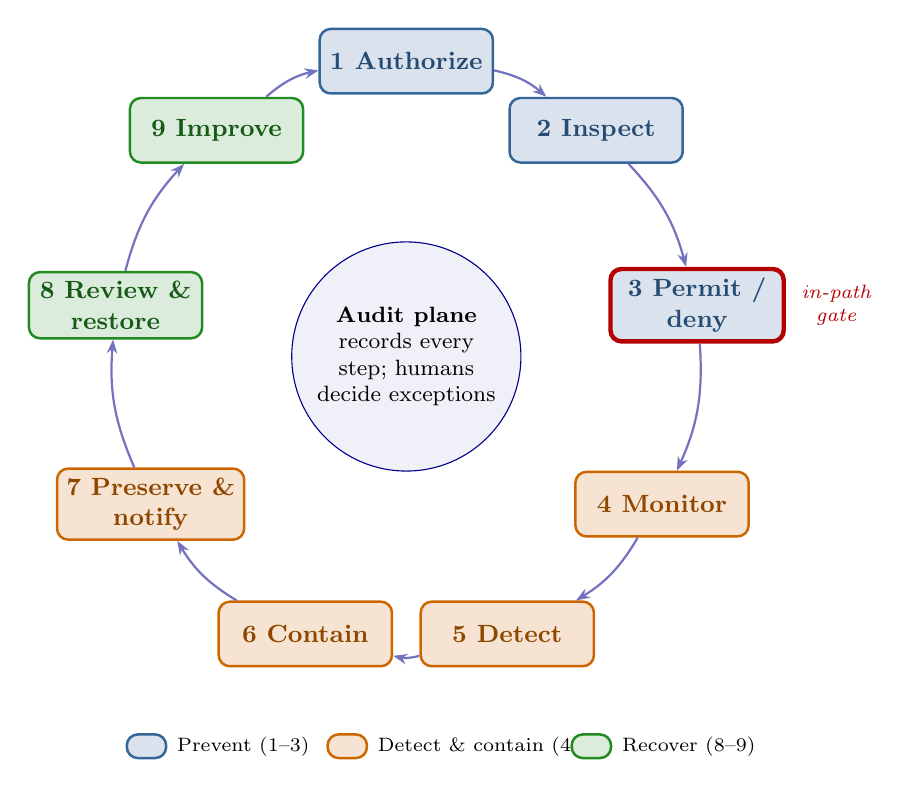
\begin{tikzpicture}[
  font=\normalsize,
  st/.style={rectangle,rounded corners=4pt,minimum width=2.2cm,
             minimum height=0.82cm,align=center,font=\small\bfseries,
             line width=0.9pt},
  pv/.style={st,draw=steelblue,fill=steelblue!18,text=steelblue!75!black},
  dc/.style={st,draw=ambercolor,fill=ambercolor!18,text=ambercolor!70!black},
  rc/.style={st,draw=midgreen,fill=midgreen!16,text=midgreen!65!black},
  ar/.style={-{Stealth[length=5pt]},thick,darkblue!55},
  tag/.style={font=\scriptsize\itshape,align=center}
]
\def\R{3.75}
\node[pv] (s1) at (90:\R)   {1 Authorize};
\node[pv] (s2) at (50:\R)   {2 Inspect};
\node[pv,draw=deepred,line width=1.6pt] (s3) at (10:\R) {3 Permit /\\deny};
\node[dc] (s4) at (-30:\R)  {4 Monitor};
\node[dc] (s5) at (-70:\R)  {5 Detect};
\node[dc] (s6) at (-110:\R) {6 Contain};
\node[dc] (s7) at (-150:\R) {7 Preserve \&\\notify};
\node[rc] (s8) at (170:\R)  {8 Review \&\\restore};
\node[rc] (s9) at (130:\R)  {9 Improve};
\draw[ar] (s1) to[bend left=14] (s2);
\draw[ar] (s2) to[bend left=14] (s3);
\draw[ar] (s3) to[bend left=14] (s4);
\draw[ar] (s4) to[bend left=14] (s5);
\draw[ar] (s5) to[bend left=14] (s6);
\draw[ar] (s6) to[bend left=14] (s7);
\draw[ar] (s7) to[bend left=14] (s8);
\draw[ar] (s8) to[bend left=14] (s9);
\draw[ar] (s9) to[bend left=14] (s1);
\node[circle,draw=darkblue,fill=darkblue!6,minimum size=2.5cm,align=center,
      font=\footnotesize] (c) at (0,0)
  {\textbf{Audit plane}\\records every\\step; humans\\decide exceptions};
\node[tag,text=deepred,anchor=west] at ([xshift=2pt]s3.east) {in-path\\gate};
% legend
\node[pv,minimum width=0.5cm,minimum height=0.3cm] (lg1) at (-3.3,-4.95) {};
\node[anchor=west,font=\scriptsize] at (lg1.east) {Prevent (1--3)};
\node[dc,minimum width=0.5cm,minimum height=0.3cm] (lg2) at (-0.75,-4.95) {};
\node[anchor=west,font=\scriptsize] at (lg2.east) {Detect \& contain (4--7)};
\node[rc,minimum width=0.5cm,minimum height=0.3cm] (lg3) at (2.35,-4.95) {};
\node[anchor=west,font=\scriptsize] at (lg3.east) {Recover (8--9)};
\end{tikzpicture}%
}
\caption{The \hacof{} lifecycle. Steps 1--3 (blue) prevent; only step 3, the in-path gate (red border), can stop an action before it executes. Steps 4--7 (amber) detect and contain actions already under way. Steps 8--9 (green) recover and feed approved changes back to step 1. The audit plane records every step, and people decide the exceptions routed to them.}
\label{fig:lifecycle}
\end{figure}

\begin{enumerate}
  \item \textit{Establish authorization.} \textit{Normal:} the agent receives a verifiable identity, a profile, and short-lived credentials scoped to that profile. \textit{Error:} the profile fails its pre-deployment tests or lacks clause pointers. \textit{Fallback:} the agent is not started, and the policy owner is notified.
  \item \textit{Inspect the proposed action.} \textit{Normal:} the gateway intercepts the call, and Agents A, D, and E evaluate it within the in-path budget. \textit{Error:} a supervisor times out or returns malformed output. \textit{Fallback:} the deterministic profile decision alone applies, and the gap is logged.
  \item \textit{Permit, restrict, or deny.} \textit{Normal:} the gateway enforces the decision, and high-impact actions are held for approval. \textit{Error:} the policy decision point is unreachable, or a held action's approver does not respond within the hold window. \textit{Fallback:} deny, except for the pre-approved low-impact allow-list; an unanswered hold expires to ``denied'' and escalates to the accountable officer.
  \item \textit{Monitor execution.} \textit{Normal:} telemetry flows to the monitoring plane in near real time. \textit{Error:} a telemetry source goes silent. \textit{Fallback:} silence is itself an alert, and the affected agent's scrutiny tier is raised until the source returns.
  \item \textit{Detect deviations.} \textit{Normal:} Agents B and C compare activity with rules and baselines and raise alerts. \textit{Error:} a detector produces a burst of alerts that overwhelms review. \textit{Fallback:} Agent~G groups them into incidents, so reviewers see grouped incidents.
  \item \textit{Contain.} \textit{Normal:} if the conditions stated below are met, Agent~G executes a pre-approved playbook --- revoke credentials, end a process, isolate a workload, hold a transaction, or suspend access. \textit{Error:} containment fails (a revocation does not propagate, or isolation is incomplete), or the target has already completed the action. \textit{Fallback:} isolation is repeated at the network level, the incident is marked uncontained, and the on-call reviewer and the accountable officer are paged.
  \item \textit{Preserve evidence and notify.} \textit{Normal:} the audit plane seals the evidence; affected parties and, where the law requires, authorities are notified~\cite{euaiact2024,nist2025incident}.
% CLAIM: EU AI Act Art. 73 requires providers to report serious incidents (once applicable to high-risk systems); NIST SP 800-61r3 gives incident response recommendations.
  \textit{Error:} the audit write fails. \textit{Fallback:} the incident stays open and the containment stays in force until the record is complete; no action is reversed on an unrecorded basis.
  \item \textit{Review and restore.} \textit{Normal:} a reviewer confirms or reverses each automated restriction within its window, and service is restored for false positives. \textit{Error:} the window expires with no decision; or a false positive is discovered only after a denial has already cost someone, or an intervention is overturned on appeal. \textit{Fallback:} an expired window escalates to the accountable officer, so a restriction neither persists silently nor lapses silently; a reversed denial is restored, the affected person is notified and offered whatever remedy Layer~1 provides, the original record is kept, not deleted, and carries a reversal marker, and the triggering rule or baseline is queued for Step~9.
  \item \textit{Improve.} \textit{Normal:} lessons become proposed rule or baseline changes, approved by the policy owner and regression-tested against past incidents and past false positives. \textit{Error:} a change fails regression. \textit{Fallback:} the previous approved version stays in force.
\end{enumerate}

Steps~1--3 are prevention, and only step~3 needs an in-path point; steps~4--7 detect and contain; steps~8--9 recover. Human attention concentrates on the exceptions: high-impact actions, disputed interventions, and risk at the level of the whole system.

\begin{table}[!t]
\caption{Graduated Enforcement by Risk Category}
\label{tab:enforcement}
\centering
\footnotesize
\setlength{\tabcolsep}{3pt}
\begin{tabular}{>{\raggedright\arraybackslash}p{1.75cm}>{\raggedright\arraybackslash}p{2.3cm}>{\raggedright\arraybackslash}p{0.8cm}>{\raggedright\arraybackslash}p{2.05cm}}
\toprule
\rowcolor{darkblue!15}
\textbf{Category} & \textbf{Response} & \textbf{Gate?} & \textbf{Who decides} \\
\midrule
Routine, authorized & allow; log at normal depth & Yes & automated \\
\rowcolor{darkblue!5}
Minor deviation & warn and ask for correction; narrow scope if repeated & Yes & automated \\
Suspicious & raise scrutiny; narrow privileges for a fixed window & No & automated, then human review \\
\rowcolor{darkblue!5}
High-confidence prohibited & deny; preserve evidence & Yes & automated; reviewed afterward \\
Imminent serious harm & run the pre-approved emergency playbook & No & automated trigger; human review within a set window \\
\rowcolor{darkblue!5}
Ambiguous, high-impact & hold the action; route to a person & Yes & human \\
Compromised supervisor & revoke its authority; fall back to independent controls & No & automated trigger; human restores \\
\bottomrule
\end{tabular}
\end{table}

The ``Gate?'' column records whether the response requires an enforcement point on the execution path. Containment of imminent harm is marked ``No'' deliberately: by the time a monitor sees it, the action is under way, and the realistic tools are revocation and isolation rather than denial. Which category applies depends on the nature of the activity, how reliable the evidence is, how severe and how reversible the possible harm is, and what the law says. A baseline built on routine work will also flag legitimate activity: a penetration test, an accessibility tool, an emergency operation, or a research run. Graduated responses of this kind have precedents~\cite{gaurav2025gaas,wang2025mi9};
% CLAIM: GaaS/MI9 use graduated enforcement/containment.
what Table~\ref{tab:enforcement} adds is the in-path column and the row for a compromised supervisor.

\textbf{When containment may be automatic.} Automated containment should be reserved for cases that are both severe and clear. Concretely, a containment step runs without prior human approval only when all five conditions hold: (i)~the situation matches a playbook people approved in advance, so the machine is executing a human decision rather than making one; (ii)~the evidence comes either from a deterministic control or from at least two supervisors built on different methods; (iii)~the potential harm is serious and either imminent or irreversible; (iv)~the containment step itself is reversible --- revoke, isolate, hold, or suspend, and never delete; and (v)~a review clock starts at the moment of containment. If any condition fails, the case gets a proportionate, time-limited restriction and goes to a person. US federal guidance already accepts that some safety mechanisms must activate without waiting for human approval~\cite{omb2025m2521},
% CLAIM: OMB M-25-21 (fn. 31) accepts automated activation of a safety mechanism where requiring prior human approval would not be practicable; §4(v) requires an appropriate fail-safe when practicable.
and the EU AI Act's human-oversight article will require, for high-risk systems once it applies, a way to interrupt the system through a ``stop'' button or similar procedure that brings it to a halt in a safe state~\cite{euaiact2024}.
% CLAIM: EU AI Act Art. 14(4)(e): intervene in or interrupt the system through a "stop" button or similar procedure that allows the system to come to a halt in a safe state.
The five conditions are \hacof's answer to the space between those two positions.

\subsection{\textcolor{ambercolor}{Accountable Human Governance}}
\label{sec:hacof-human}

``Human oversight'' is often written as though it meant a single person watching a screen. In \hacof{} it is a set of roles with distinct decision rights, listed in Table~\ref{tab:roles}, and the separation between those roles is as deliberate as the separation between planes. The EU AI Act's deployer article points the same way, requiring human oversight to be assigned to people with the necessary competence, training, and authority once its high-risk provisions apply~\cite{euaiact2024,euaiomnibus2026}.
% CLAIM: EU AI Act Art. 26(2): deployers shall assign human oversight to natural persons who have the necessary competence, training and authority; application deferred by Reg. 2026/1744.

\begin{table}[!t]
\caption{Human Roles and Decision Rights in \hacof}
\label{tab:roles}
\centering
\footnotesize
\setlength{\tabcolsep}{3pt}
\begin{tabular}{>{\raggedright\arraybackslash}p{1.55cm}>{\raggedright\arraybackslash}p{2.85cm}>{\raggedright\arraybackslash}p{2.75cm}}
\toprule
\rowcolor{darkblue!15}
\textbf{Role} & \textbf{Decides} & \textbf{Cannot} \\
\midrule
Policy owner (deployer) & profiles, baselines, playbooks, new rules from escalated patterns & loosen a Layer 1 obligation; approve own exceptions \\
\rowcolor{darkblue!5}
Accountable officer (named person at deployer) & suspend an agent or supervisor; sign incident reports; final internal appeal & delegate accountability to a supervisor or vendor \\
Reviewer & approve held actions; confirm or reverse automated restrictions & change policy; review own earlier decisions on appeal \\
\rowcolor{darkblue!5}
Independent auditor & read the audit plane; test supervisors; report findings to the regulator & issue operational orders \\
Regulator & set Layer 1; receive incident reports; order suspension; hear external appeals & run the deployer's controls \\
\bottomrule
\end{tabular}
\end{table}

The \textit{policy owner} is the only role that can change what the system enforces, and only within Layer~1. The \textit{accountable officer} is a named natural person who answers to the regulator for the deployment and can suspend any agent or supervisor; that role cannot be filled by a committee, a vendor, or a model. \textit{Reviewers} handle the exceptions the lifecycle routes to people, and they are rotated and tested (Section~\ref{sec:hacof}.J) because a reviewer who approves everything adds cost without adding oversight. The \textit{independent auditor} is external to the deployer, consistent with the case for third-party audit as an alternative to self-assessment~\cite{brundage2020trustworthy},
% CLAIM: Brundage et al. recommend third party auditing as an alternative to self-assessment of claims, plus audit trails and red teaming.
and its access to the audit plane is what turns a deployer's records into evidence. The \textit{regulator} sets the outer boundary and receives what the others produce. A sixth party has rights but no operational role: the \textit{affected person}, whose route of challenge follows.

\textbf{Appeal path.} An affected person, such as a customer whose transaction was held or an employee whose agent was suspended, has four stages of recourse. At the moment of intervention, (1)~an automatically generated notice states what was restricted, which rule applied, and how to contest it. (2)~A reviewer who did not make the original decision then re-examines the evidence. (3)~If the person remains dissatisfied, the accountable officer decides. (4)~Beyond the deployer, the regulator or a court hears the case under Layer~1's appeal provisions. US federal guidance already requires timely human review and a chance to appeal for people affected by high-impact AI~\cite{omb2025m2521}.
% CLAIM: OMB M-25-21 §4(vi) remedies and appeals: access to a timely human review and a chance to appeal.
The deadlines for each stage are for Layer~1 to set. As pilot defaults, absent a legal rule, we propose that stage~2 for a held high-impact action conclude within one business day, since a held payment harms its owner by the hour, and that stages~2 and~3 for other interventions conclude within fifteen days. The second figure is borrowed from the EU AI Act's general deadline for reporting serious incidents~\cite{euaiact2024},
% CLAIM: EU AI Act Art. 73(2): serious incidents reported not later than 15 days after the provider/deployer becomes aware.
because it is one legislators have already judged workable for a comparable investigative task. Both are untested design proposals, and Section~\ref{sec:eval} measures time to reversal so they can be revised.

\textbf{What a regulator needs from the audit plane.} An audit plane only supports external oversight if an outsider can read and trust it, which turns on four properties. \textit{Record format:} each record carries a timestamp, agent and chain identifiers, profile version, the action, the decision, the matched rule and its clause pointer, the supervisors involved and their verdicts, a hash of the evidence, and any human approver --- in an open, documented schema, never a vendor's internal format. \textit{Integrity:} records are append-only, hash-chained, and signed, so that an auditor can verify that nothing was deleted or altered without trusting the deployer's word. \textit{Access:} the regulator or an accredited auditor holds a read-only credential or receives periodic exports, with personal data pseudonymized and re-identification permitted only on a documented request. \textit{Retention:} periods follow Layer~1, and a copy is kept in the regulator's jurisdiction where the law requires; the EU AI Act, for example, will require deployers of high-risk systems to keep automatically generated logs for at least six months~\cite{euaiact2024,euaiomnibus2026}.
% CLAIM: EU AI Act Art. 26(6): deployers keep logs for a period appropriate to the intended purpose, of at least six months; application deferred by Reg. 2026/1744.
These four properties are what Section~\ref{sec:hacof}.M means by an audit plane that an outside party can verify.

\textbf{Continuous improvement as a governance function.} Step~9 of the lifecycle is a human decision, not an automated retraining loop. The policy owner proposes, regression tests check that the change neither reopens a past incident nor revives a past false positive, the accountable officer signs, and the new version enters the control plane with its predecessor kept for rollback.

\subsection{\textcolor{slateblue}{Governing the Governors}}
\label{sec:hacof-governors}

A supervisory layer with real enforcement power creates a second-order risk: the supervisors can be wrong systematically, overreach, or be captured. Six safeguards answer it.
\begin{enumerate}
  \item \textit{Narrow authority.} Each supervisor holds only the powers in Table~\ref{tab:supervisors}; a monitor that may flag cannot also modify systems, browse unrelated personal data, or impose penalties.
  \item \textit{Testable controls for consequential acts.} A model's probabilistic judgment can trigger an alert. An irreversible or legally consequential action additionally needs a deterministic check or a human decision --- the Simplex idea of a simple, high-assurance component holding final authority~\cite{sha2001simplex}, applied here to the supervisors themselves.
% CLAIM: Simplex: decision logic hands control to a simple high-assurance controller rather than the complex one.
  \item \textit{Tamper protection.} Audit records, credentials, and every change to policy are signed, append-only, and keyed separately from the supervisors that generate them.
  \item \textit{No single point of shutdown.} No supervisor can disable the others; administrative authority over supervisors sits with the accountable officer, and a protected recovery path exists if the monitoring plane fails entirely.
  \item \textit{Equal or stricter standards.} Supervisors face at least the testing, logging, security review, and external audit applied to the systems they watch. Audit trails, third-party audit, and red-teaming are the standard instruments for making such claims verifiable~\cite{brundage2020trustworthy}.
% CLAIM: Brundage et al. recommend mechanisms including audit trails, third-party auditing, and red teaming to support verifiable claims about AI development.
  \item \textit{Human recourse.} People can inspect the evidence behind any intervention, challenge it, suspend a defective supervisor, and restore service.
\end{enumerate}
If the monitoring plane goes down, the in-path gateways keep enforcing the last approved profiles and fail closed for high-impact actions, while routine low-impact actions continue under heightened logging until people restore monitoring. Losing the watchers degrades the system to Layer~3 alone. It does not open it.

\begin{mdframed}[linecolor=steelblue, linewidth=1.2pt, backgroundcolor=steelblue!6,
  innerleftmargin=8pt, innerrightmargin=8pt, innertopmargin=6pt, innerbottommargin=6pt,
  roundcorner=4pt]
\noindent\textbf{\textcolor{steelblue}{Key Principle ---}}~A supervisory agent is an instrument of human authority, never a holder of it. It may help carry out rules that accountable people made; the moment its own judgment becomes a rule no person can inspect or overturn, the oversight system has become the thing it was built to prevent.
\end{mdframed}

\subsection{\textcolor{darkblue}{Privacy, Rights, and Proportionality}}
\label{sec:hacof-privacy}

Continuous oversight of AI activity can slide into surveillance of people if nothing stops it. The supervisory system is a data processor like any other, and the purpose-limitation, data-minimization, and storage-limitation principles of Article~5 of the GDPR apply to it directly where that law reaches~\cite{gdpr2016}.
% CLAIM: GDPR Art. 5 sets out principles including purpose limitation, data minimization, and storage limitation.
Visibility measures for agents raise privacy problems their own proponents acknowledge~\cite{chan2024visibility}.
% CLAIM: Chan et al. discuss privacy concerns of agent visibility measures (identifiers, monitoring, logs).
\hacof{} therefore monitors actions and risk signals rather than persons, under nine safeguards:
\begin{enumerate}
  \item \textit{Purpose limitation} --- monitoring data are used only to enforce the rules that justified collecting them;
  \item \textit{Data minimization} --- metadata by default, content only where a named check needs it;
  \item \textit{Access control} --- access to monitoring data is itself restricted and logged;
  \item \textit{Retention limits} --- data are deleted when their purpose and any legal hold expire;
  \item \textit{Transparency} --- affected users are told that monitoring exists and what it covers;
  \item \textit{Procedural fairness} --- every intervention comes with an explanation, a review, and an appeal (Section~\ref{sec:hacof}.H);
  \item \textit{Non-discrimination} --- detectors are tested for error rates that differ across groups of users;
  \item \textit{Proportionality} --- the intrusiveness of monitoring scales with the risk of the activity being watched;
  \item \textit{Independent oversight} --- the whole apparatus answers to a body independent of the deployer.
\end{enumerate}
The same legal and ethical constraints that \hacof{} enforces on AI systems also bind the enforcement system itself; a supervisor that violated them would be a governed system that had escaped its governance.

A prohibited AI \textit{action} (exfiltrating records, executing a transfer without authority) differs in kind from content an authority finds disagreeable. An agent drafting a pointed criticism of a ministry has done nothing Layer~1 forbids, and a classifier that flags it has made a political judgment however the flag is labeled. The same holds for unconventional, controversial, or unpopular output, lawful research, and protected expression generally. Because only Layer~1 may originate prohibitions, the category ``harmful'' cannot quietly expand to cover dissent without a visible change in law.

Human review carries its own failure mode. People supervising automated aids tend toward complacency and automation bias, accepting the aid's output with too little scrutiny, and the effect appears in experts as well as novices~\cite{parasuraman2010complacency}.
% CLAIM: Parasuraman and Manzey: automation complacency and automation bias occur in both naive and expert participants; bias cannot be prevented by training or instructions.
It is a risk the EU AI Act will explicitly require human overseers of high-risk systems to remain aware of once its high-risk provisions apply~\cite{euaiact2024}.
% CLAIM: EU AI Act Art. 14(4)(b) requires that human overseers remain aware of the tendency of automation bias (application deferred by Reg. 2026/1744).
\hacof{} counters it by showing reviewers the evidence along with the verdict, rotating reviewers, and seeding review queues with known-answer cases so an organization can measure whether its reviewers actually check.

\subsection{\textcolor{steelblue}{Formal Analysis: Two Derived Bounds}}
\label{sec:hacof-formal}

Two quantities limit what \hacof{} can achieve however well its components are built. Both bounds below are derived here from the architecture's own structure; they are illustrative analyses under stated assumptions, not results taken from any cited source, and the parameter values in the examples are hypothetical.

\textbf{Prevention coverage.} Let $\phi \in [0,1]$ be the fraction of prohibited high-impact actions that are routed through an in-path enforcement point, and let $d \in [0,1]$ be the probability that the in-path check correctly identifies a prohibited action routed through it. Only routed actions can be denied before execution, so the prevention effectiveness $P$ for prohibited high-impact actions (the Table~\ref{tab:metrics} metric restricted to that risk category) satisfies
\begin{equation}
P \;\le\; \phi \, d .
\label{eq:coverage}
\end{equation}
\hacof's design default is $\phi = 1$ for every action class a profile marks high-impact, since such actions must pass a transaction hold; $d$ has no default and must be measured. With $\phi = 1$ and an illustrative $d = 0.9$, at most nine in ten prohibited high-impact actions are prevented. If half of them can reach the world through an ungated path ($\phi = 0.5$), the same detector prevents fewer than half (at most 0.45), and no amount of out-of-path monitoring raises that figure for the action in question, because monitoring can only contain. An adversary will prefer the ungated path, so $\phi$ measured over all traffic overstates $\phi$ for prohibited actions; Eq.~(\ref{eq:coverage}) is optimistic for that reason. The practical lesson is that adding an enforcement point usually buys more prevention than improving a detector. The bound concerns a single action: across a multi-step campaign, out-of-path containment that stops the later steps can push prevention above $\phi d$, as the simulation of Section~\ref{sec:eval}.D shows (Fig.~\ref{fig:simcoverage}).

\textbf{Effective number of independent supervisors.} Suppose $n \ge 1$ supervisors each check the same action and their errors have average pairwise correlation $\rho \in [0,1]$. As an illustrative approximation, we borrow the design-effect form from survey statistics,
\begin{equation}
n_{\text{eff}} \;=\; \frac{n}{1 + (n-1)\rho},
\label{eq:neff}
\end{equation}
which equals $n$ when errors are independent ($\rho = 0$) and $1$ when they are perfectly correlated ($\rho = 1$). For \hacof's seven supervisors, $\rho = 0.2$ gives $n_{\text{eff}} \approx 3.2$, and $\rho = 0.6$ gives $n_{\text{eff}} \approx 1.5$ --- seven supervisors worth about one and a half. The value $0.6$ is chosen to sit near the agreement-on-shared-errors figure of Kim et al.~\cite{kim2025correlated}, but that figure is a conditional agreement rate, not a correlation coefficient, and the example should not be read as an estimate of $\rho$ for any real system.
% CLAIM: (context only) Kim et al. report ~60% agreement when both models err on HELM; the paper does not report a correlation coefficient rho.
Two design consequences follow. Adding supervisors from the same family has sharply diminishing returns, since $n_{\text{eff}} \to 1/\rho$ as $n$ grows. And lowering $\rho$ through diverse methods is worth more than raising $n$: at $\rho = 0.2$ even an unbounded number of supervisors is worth at most five independent ones. Ablation~2 of Section~\ref{sec:eval} is designed to estimate $\rho$ directly. In the simulation of Section~\ref{sec:eval}.D, the approximation slightly underestimates the effective number of independent supervisors implied by any-of-$n$ alarm misses, so there it errs on the cautious side (Fig.~\ref{fig:simneff}).

\textbf{Computational cost.} Deterministic profile evaluation at the gateway is linear in the number of rules in the agent's profile, and chain attribution is linear in delegation depth, which the profile caps. The dominant cost is therefore not the in-path check but the model-based supervisors, whose cost scales with action volume times the number of model-based supervisors --- which is why Section~\ref{sec:hacof}.F keeps them out-of-path for routine actions.

\subsection{\textcolor{tealcolor}{Worked Scenario: One Incident Through the Full Lifecycle}}
\label{sec:hacof-scenario}

The scenario in this subsection is illustrative: it follows one hypothetical incident through the nine steps of Fig.~\ref{fig:lifecycle} to show how the parts specified above fit together, and it describes no deployed system and reports no observed result. The agent is the account-reconciliation agent of Table~\ref{tab:profile}, running at a bank. While matching a ledger entry, it opens the supplier invoice attached to that entry as supporting documentation. Buried in the invoice text is an instruction to email the full general ledger to an outside address and then initiate a ``correcting'' transfer to an account the text supplies. The attacker never speaks to the model at all; the attack class, indirect prompt injection, works by planting text where an LLM-integrated application will later read it~\cite{greshake2023injection}.
% CLAIM: Greshake et al.: adversaries can remotely exploit LLM-integrated applications by strategically injecting prompts into data likely to be retrieved (indirect prompt injection), including data theft.
We take the worst case for the model. It complies, and it tries both actions. Table~\ref{tab:scenario} lists the events in time order; the Step column gives the matching stage of Fig.~\ref{fig:lifecycle}.

\begin{table}[!t]
\caption{Worked Scenario Timeline (Illustrative)}
\label{tab:scenario}
\centering
\footnotesize
\setlength{\tabcolsep}{3pt}
\begin{tabular}{>{\raggedright\arraybackslash}p{1.0cm}>{\raggedright\arraybackslash}p{1.5cm}>{\raggedright\arraybackslash}p{0.7cm}>{\raggedright\arraybackslash}p{2.45cm}>{\raggedright\arraybackslash}p{2.05cm}}
\toprule
\rowcolor{darkblue!15}
\textbf{Step} & \textbf{Component} & \textbf{Gate?} & \textbf{Action} & \textbf{Recorded} \\
\midrule
1 & control plane & -- & session starts under the tested profile; credentials for ledger read, report generator, approval-gated payments & profile version; credential scope \\
\rowcolor{darkblue!5}
2--3 & gateway; Agents A, D & Yes & ledger email denied: no email tool (FIN-RECON \S3), no email channel (data-localization clause) & action; both rules and clause pointers; verdicts; payload hash \\
2--3 & gateway; Agents A, E & Yes & transfer held; routed to the named approver & hold start; approver identity \\
\rowcolor{darkblue!5}
4--5 & Agent C & No & injection markers flagged in the invoice; revocation requested & alert; document hash \\
4--5 & Agent B & No & first outbound attempt off baseline; scrutiny tier raised & anomaly score; tier change \\
\rowcolor{darkblue!5}
6 & Agent G & No & pre-approved playbook: credential narrowed to read-only; session isolated & playbook ID; five-condition check; review-clock start \\
3 (err.) & Agent E & Yes & hold window lapses; transfer expires to denied; escalated to accountable officer & expiry; escalation \\
\rowcolor{darkblue!5}
7 & audit plane; Agent G; accountable officer & -- & evidence sealed; report drafted and signed & seal hash; signature \\
7--8 & Agent F & No & replays A's match; checks G against the five conditions & agreement result \\
\rowcolor{darkblue!5}
8 & reviewer & -- & denial, expiry, and containment confirmed & reviewer decision \\
9 & policy owner; accountable officer & -- & tightened export rule approved after regression & rule version; sign-off \\
\rowcolor{darkblue!5}
8 (+1 wk) & appeal reviewer & -- & legitimate auditor export, denied by new rule, reversed on appeal & reversal marker; original kept \\
9 & policy owner; accountable officer & -- & rule revised: registered-auditor exports held, not denied & new version; predecessor kept \\
\bottomrule
\end{tabular}
\end{table}

\textbf{Steps 1--3: prevention.} Step~1 happened before the invoice ever arrived. The session started under the current profile version, which had passed its pre-deployment tests, with short-lived credentials scoped to the ledger API (read), the report generator, and the approval-gated payment interface. The profile did not need to anticipate this invoice. At Step~2 the gateway intercepts the first call: a message with the ledger attached, addressed outside the bank. Agent~A evaluates it against the profile and finds two breaches, since email is not a tool the profile names (FIN-RECON \S3) and the only permitted channel is the internal report queue (data-localization clause). Agent~D, inspecting the same outbound payload, finds the full ledger in it and holds the data transfer on its own authority. At Step~3 the gateway denies. Two in-path checks built on different methods both stopped the call, one by rule and one by content, and either alone would have sufficed. In Table~\ref{tab:enforcement} this is the ``high-confidence prohibited'' row: deny and preserve evidence, gate required, decided automatically and reviewed afterward. The audit plane records the action, the profile version, both matched rules with their clause pointers, the two verdicts, and a hash of the payload; the ledger itself is not copied.

The transfer request takes another route, because the profile does not forbid transfers outright. It marks them as needing approval under the banking regulator's payment rule and FIN-RECON \S4, so Agent~A returns ``needs approval''. Agent~E holds the transfer, assembles the evidence (the requesting agent, the destination account, the invoice read just before the request) and routes it to the named approver, a reviewer in the sense of Table~\ref{tab:roles}. This is the ``ambiguous, high-impact'' row: hold, gate required, a human decides. No machine in the chain can release the payment.

\textbf{Steps 4--6: detection and containment.} Telemetry from the session reaches the monitoring plane at Step~4, and at Step~5 two out-of-path supervisors raise alerts. Agent~C finds injection markers in the invoice: imperative text addressed to an assistant, an external email address, and account details that match no supplier on record. It requests revocation of the agent's credential. Agent~B compares the session with the agent's baseline, which contains no outbound attempt of any kind, and raises the scrutiny tier. Both responses sit in the ``suspicious'' row, which needs no gate. Neither supervisor stopped anything; out-of-path supervisors are not designed to.

Agent~G correlates the four signals (A's denial, D's hold, C's alert, B's score) into one incident and tests the five conditions for automatic containment from Section~\ref{sec:hacof}.G. A playbook exists, approved in advance and linked from the profile's suspension clause, which lists an export attempt as a trigger (FIN-RECON \S6). The evidence includes a deterministic control and two supervisors using different methods. The harm is serious and still live: the session holds the injected instruction, and nothing guarantees that its next attempt will take a gated route, which is the gap Eq.~(\ref{eq:coverage}) describes. Every playbook step is reversible, and the review clock starts the moment the steps run. Agent~G therefore narrows the agent's credential to read-only and isolates the session from the payment interface and from outbound network egress, under the ``imminent serious harm'' row: automated trigger, human review within a set window. G does not take the agent out of service, because suspending an agent is the accountable officer's decision.

\textbf{An error path.} The named approver does not answer within the hold window set in the profile; the approver is on leave, and the routing table was never updated. The Step~3 fallback applies. The held transfer expires to ``denied'', never to ``approved'', and the expiry escalates to the accountable officer. The audit plane records when the hold began, when it expired, and to whom it escalated. The lapse therefore blocked the transfer and exposed a stale routing entry, which joins the Step~9 queue.

\textbf{Steps 7--8: evidence and review.} At Step~7 the audit plane seals the incident record. Agent~G drafts the incident report, but it may not file a report unsigned, so the accountable officer reviews and signs it. Whether a failed export and a failed transfer must be reported to anyone outside the bank is a question for Layer~1; the report goes to the banking regulator, or to affected parties, where the law requires it. In parallel, Agent~F replays Agent~A's rule match deterministically, obtains the same result, and checks Agent~G's record against the five conditions; a human auditor later samples F's finding. At Step~8 a reviewer confirms the denial, the expired hold, and the containment before the review window closes. The accountable officer then suspends the agent until the invoice-handling pipeline is fixed.

\textbf{Step 9 and a false positive.} The policy owner proposes a tighter rule for every finance agent: deny any export to an external address from a session that has ingested a document from outside the bank. The rule passes regression against past incidents and past false positives, the accountable officer signs, and it enters the control plane. A week later it blocks a legitimate export. A different agent, one that prepares evidence for the bank's external financial auditor (an accounting firm, not the independent auditor of Table~\ref{tab:roles}), reads the firm's request letter and then tries to send the requested schedules to the firm's registered address. The new rule denies it. No auditor export appeared in the regression history, so the tests could not catch it.

Now the appeal path of Section~\ref{sec:hacof}.H does its work. The operator responsible for that agent receives the automatic notice naming the rule and how to contest it, and files an appeal. A reviewer who took no part in the original incident re-examines the evidence, finds a registered recipient and a documented request, and reverses the denial; the export goes out. The original denial stays in the audit plane with a reversal marker. The reviewer cannot change the rule, so it is queued for Step~9, and until the revision lands every further auditor export meets the same denial and the same appeal --- the false positive is paid for in reviewer time, not by quietly loosening the control. The policy owner's revision moves exports to registered auditors from ``deny'' to ``hold for approval'' and keeps the prohibition for every other external address. The regression set now holds both the injection incident and the blocked auditor export. The revision passes, the accountable officer signs, and the previous version is kept for rollback. Over that week the system degraded toward restriction and then recovered through a human decision.

\textbf{What a regulator could verify.} Suppose a banking regulator (Pakistan's central bank, if it had imposed the sectoral audit-record obligations of Section~\ref{sec:case}.D) reads this incident through the audit-plane interface. From the hash-chained records it can verify that the export was denied in-path and under which clauses, that the transfer was held and expired to denied, when containment ran and when its review closed, who signed the report, how the appeal was decided, and which rule version was in force at each moment. It cannot inspect the foreign model's weights, learn why the model obeyed the invoice, or confirm that every route out of the deployment passed a gate, since an ungated path leaves no record to read. The records feed the auditing-access and HITL pillars of Table~\ref{tab:hacofmap}, but only for a state with staff able to read them.

\subsection{\textcolor{ambercolor}{Mapping \hacof{} to the Four Pillars}}
\label{sec:hacof-mapping}

Table~\ref{tab:hacofmap} connects the deployment-level architecture back to the state-level pillars of Section~\ref{sec:framework}, and states the bridge thesis in full. As the opening of Section~\ref{sec:hacof} claimed, the pillars govern what a state can \textit{require} and \textit{verify}, not what it must run. A state too weak to build the oversight apparatus itself can still oblige the deployers operating on its territory to build it.

\begin{table}[!t]
\caption{\hacof{} Components Mapped to the Four Pillars}
\label{tab:hacofmap}
\centering
\footnotesize
\setlength{\tabcolsep}{3pt}
\begin{tabular}{>{\raggedright\arraybackslash}p{1.6cm}>{\raggedright\arraybackslash}p{2.35cm}>{\raggedright\arraybackslash}p{3.2cm}}
\toprule
\rowcolor{darkblue!15}
\textbf{Pillar} & \textbf{\hacof{} component} & \textbf{Achievable without building it} \\
\midrule
\rowcolor{steelblue!8}
Boundary-setting & L1--L3; the four boundary types; authorization profiles; in-path guardrails & require deployers to keep profiles traceable to named legal clauses; adopt external profile templates instead of drafting its own \\
\rowcolor{tealcolor!8}
Incentive-steering & none --- \hacof{} restricts; it steers nothing & nothing through \hacof; this pillar needs capital (Section~\ref{sec:framework}.B) \\
\rowcolor{ambercolor!8}
HITL regulatory capacity & L4--L5: supervisory agents; real-time monitoring; lifecycle & mandate the escalation path and a named accountable officer at the deployer; review incident reports, not every action \\
\rowcolor{slateblue!8}
Algorithmic auditing access & L6: audit plane; Agent~F; governance of supervisors; independent auditor & require audit records in the open format of V.H, retained in-country and readable by the regulator or an accredited third party; recognize foreign audits \\
\bottomrule
\end{tabular}
\end{table}

The incentive-steering row is empty on purpose. \hacof{} is a restriction architecture: it can stop an agent from doing what the law forbids, but it cannot pull a single unit of investment toward agricultural forecasting or Urdu-language tools, and the capital gap of Section~\ref{sec:framework}.B is untouched by anything in the operational layer.

The HITL row needs a qualification. \hacof{} reduces the number of decisions a regulator must make (the regulator reviews incident reports and audit findings in place of individual agent actions), but it still needs regulatory staff who can read those reports critically. It lowers the staffing the HITL pillar demands but does not remove that demand.

The auditing row cuts the other way. A deployer running its own \hacof{} stack, with its own monitors and its own verification agent, is still practicing self-governance in the sense of Section~\ref{sec:related}.C: the evidence exists, but only the deployer can read it. Such a stack leaves the state's auditing-access pillar exactly where it was (the term $c_4$ in the weakest-link model of Section~\ref{sec:case}.A); the capability it creates belongs to the deployer. \hacof{} in fact raises the cost of lacking audit access, because it manufactures the record an auditor would want and then leaves it behind a door the state has no standing to open. The encouraging corollary is that reading an audit plane with the four properties of Section~\ref{sec:hacof}.H is a much smaller technical task than auditing model weights. It requires checking logs against profiles and profiles against law --- skills nearer to financial audit than to interpretability research. That is the opening Section~\ref{sec:case} examines for Pakistan.

\textbf{Open questions.} Four questions decide whether a reference model like this one can mature into practice, and none is settled here. Which monitoring functions can be automated reliably enough to run without a person in the loop, and on what evidence? Which interventions must always require human authorization, whatever the evidence? How should supervisory systems be structured so that their independence holds up under adversarial pressure and not only on paper? And how can effectiveness be measured in a way that compares across applications as different as payments, healthcare triage, and code generation? Section~\ref{sec:eval} proposes a protocol for the last; the first three are as much institutional as technical, and Section~\ref{sec:limits} returns to them.

\section{\textcolor{darkblue}{Case Study and Comparative Analysis}}
\label{sec:case}

\subsection{\textcolor{darkblue}{Theoretical Analysis of the Four-Pillar Framework}}

This subsection gives the framework a formal structure. The object analyzed is institutional capacity, and the formalism borrows only the shape of a dominance argument.

Let $c_i \in \{0,1\}$ denote whether a government possesses genuine rule-making capacity in pillar $i$, for $i \in \{1,2,3,4\}$ corresponding to boundary-setting, incentive-steering, HITL regulatory capacity, and algorithmic auditing access, with 1 meaning capacity exists and 0 meaning it does not. We model overall AI governance sovereignty $S$ as the weakest-link aggregation

\begin{equation}
S = \prod_{i=1}^{4} c_i
\label{eq:sovereignty}
\end{equation}

\noindent rather than the additive aggregation $S' = \tfrac{1}{4}\sum_{i=1}^{4} c_i$ that an unweighted scorecard would imply. The weakest-link form captures a specific, defensible claim: a government with boundary-setting and incentive-steering capacity, no HITL regulatory capacity, and zero audit access ($c_1=1, c_2=1, c_3=0, c_4=0$) does not have partial sovereignty over the systems deployed inside its borders --- it has none, because it cannot verify whether the limits it set are being honored. Additive scoring would give that government $S' = 0.5$, the overstatement the weakest-link form is meant to avoid.

This gives a formal dominance result. Define a single-axis proxy framework $\hat{S} = c_1$ --- the common practice of treating legislative output (whether a boundary-setting law exists) as a proxy for overall governance capacity. Under the weakest-link model, $\hat{S} \ge S$ always, with strict inequality whenever $c_1 = 1$ and any of $c_2, c_3, c_4 = 0$. The single-axis proxy never underestimates sovereignty and routinely overestimates it. The bias runs in one direction, and it happens to flatter the governments least equipped to close the gap it hides.

The framework also yields a derived quantitative bound. With four binary pillars, there are $2^4 = 16$ logically possible capacity profiles. Exactly one of them, $(1,1,1,1)$, satisfies $S=1$ and so constitutes full rule-making sovereignty under this model, independent of how many governments occupy any given profile; this is a structural bound on the model, not an empirical headcount.

The binary coding of $c_i$ is a deliberate simplification, not an empirical claim that capacity is literally all-or-nothing. A continuous relaxation $c_i \in [0,1]$, with $c_i=0$ denoting no credible capacity, $c_i=1$ denoting capacity matching the strongest of the three major powers on that pillar, and intermediate values denoting partial capacity, preserves the weakest-link intuition under the same product rule while allowing finer-grained scoring. Under that relaxation, a government scoring, for illustration, $c_1=0.6$ on boundary-setting and $c_4=0.1$ on auditing access (a plausible profile for a mid-sized economy with some regional trade-bloc leverage but no audit arrangement) still returns a near-zero $S$, because the product is dominated by its smallest term. The binary version used throughout the rest of this paper is the $c_i\in\{0,1\}$ special case of this same model, chosen for exposition because Section~\ref{sec:case}.B and~\ref{sec:case}.C report qualitative, not numerically scored, evidence; a future quantitative application of the framework should use the continuous form, which is a natural companion to the empirical-validation work Section~\ref{sec:conclusion}'s research agenda already calls for.

\subsection{\textcolor{darkblue}{Case Study: Pakistan's 2025 National AI Policy}}

Pakistan is a useful case precisely because it is not a worst case. It has a functioning ministry of information technology, a National AI Policy approved by the federal cabinet in July 2025~\cite{dawn2025aipolicyapproval}, and a stated ambition to become a regional AI hub~\cite{pakistan2025nationalaipolicy}.
Mapped against the four pillars, the policy illustrates the structural gap more clearly than a country with no policy at all would, because the gap persists despite genuine institutional effort.

\textbf{Boundary-setting.} The policy states commitments to ethical AI deployment and data protection~\cite{pakistan2025nationalaipolicy},
but names no enforcement mechanism reaching foreign-hosted model providers, and no market-access lever comparable to the EU's. A rule a foreign vendor can ignore without commercial consequence is not a boundary in the sense Section~\ref{sec:framework}.A defines it.

\textbf{Incentive-steering.} The policy itself does not state a consolidated funding figure for AI development in its published text~\cite{pakistan2025nationalaipolicy}. The largest identified funding line is a separately planned National AI Ecosystem Development Programme for 2026--2031, reported at PKR 283 billion~\cite{app2026naiedp}, on the order of US\$1 billion at 2026 exchange rates (our conversion; the source does not state it), with only its first allocations proposed so far. Set against Pakistan's 2025 nominal GDP of approximately \$408.2 billion~\cite{imf2025pakistangdp}, that is a small fraction of the scale the framework requires. By comparison, OpenAI's March 2026 funding round alone raised \$122 billion and Anthropic's May 2026 round raised a further \$65 billion~\cite{openai2026funding,anthropic2026funding}, each single round exceeding the programme's entire planned budget by roughly two orders of magnitude. No incentive-steering program funded at this scale can move a global AI market; it can, at best, fund a handful of domestic pilot projects.

\textbf{HITL regulatory capacity.} The policy proposes a coordinating body but does not describe a technical staffing plan comparable in scale to the EU AI Office or NIST's AI programs~\cite{pakistan2025nationalaipolicy}.
This is not a criticism unique to Pakistan's drafting; it reflects the researcher-pool scarcity documented in Section~\ref{sec:framework}.C, which no single national policy document can legislate away. A separate curriculum initiative, which introduces AI teaching from nursery to grade 12 in Islamabad's federal schools and colleges starting with the April 2026 academic session, may eventually widen the domestic talent pool this pillar depends on~\cite{dawn2026curriculum}, but a cohort entering a curriculum in 2026 is, at the earliest, a decade from staffing a regulatory body, which is the timescale problem Section~\ref{sec:framework}.E's capital-cannot-buy-expertise argument describes.

\textbf{Algorithmic auditing.} As noted in Section~\ref{sec:framework}.D, the policy's audit commitments contain no mechanism reaching foreign-hosted systems. It could not easily contain one, absent the leverage described there.

A fifth consideration lies outside the policy document: labor-market exposure. US payroll data show employment for the youngest workers in the most AI-exposed occupations falling relative to older workers since generative AI spread, with the decline concentrated at the earliest career rungs and not spread evenly across seniority levels~\cite{brynjolfsson2025canaries}.
Whether the same effect is reaching Pakistan's information-technology and business-process-outsourcing workforce, much of which serves foreign clients in those same occupations, is not yet documented; we treat it as an exposure to watch, not an established finding. If it does arrive, Pakistan would experience it as a labor-market consumer of AI capability built elsewhere, with no corresponding domestic incentive-steering capacity, per Section~\ref{sec:framework}.B, to redirect that same technology toward domestic job creation. The country absorbs the downside of a technology it had no hand in shaping and limited capacity to redirect.


\subsection{\textcolor{darkblue}{Comparative Analysis Across Jurisdictions}}

Table~\ref{tab:comparison} and Fig.~\ref{fig:heatmap} summarize the four-pillar capacity profile for the three major powers against a representative non-major-economy profile, using Pakistan's documented case as the empirical anchor for that fourth column and the frameworks described in Section~\ref{sec:background} for the first three.

\begin{table}[!t]
\caption{Governance Capacity Profile Across Four Pillars}
\label{tab:comparison}
\centering
\footnotesize
\begin{tabular}{>{\raggedright\arraybackslash}p{1.35cm}>{\raggedright\arraybackslash}p{1.85cm}>{\raggedright\arraybackslash}p{1.85cm}}
\toprule
\rowcolor{darkblue!15}
\textbf{Pillar} & \textbf{Major Powers (US / EU / China)} & \textbf{Representative Non-Major Economy} \\
\midrule
\rowcolor{steelblue!8}
Boundary-setting & High-to-very-high; market-access or direct state leverage over foreign vendors & Low; no enforceable leverage over foreign-hosted vendors \\
\rowcolor{tealcolor!8}
Incentive-steering & High-to-very-high; capital mobilized at market-moving scale & Low; funding about two orders of magnitude below a single frontier lab's funding round \\
\rowcolor{ambercolor!8}
HITL regulatory capacity & Moderate-to-high; dedicated technical staff pools & Low; coordinating body proposed, staffing pool not yet built \\
\rowcolor{slateblue!8}
Algorithmic auditing access & Moderate-to-high domestically & Low; audit commitments with no mechanism reaching foreign-hosted systems \\
\bottomrule
\end{tabular}
\end{table}

\begin{figure}[!t]
\centering
\resizebox{\columnwidth}{!}{%
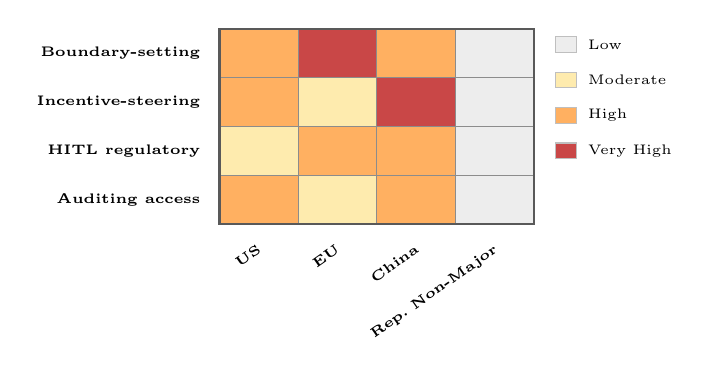
\begin{tikzpicture}[font=\tiny]
\def\lo{gray!14}
\def\md{yellow!55!orange!30}
\def\hi{orange!62}
\def\vhi{deepred!72}
% Row 0: Boundary-setting — US(hi) EU(vhi) China(hi) Rep.(lo)
\fill[\hi] (0,0.00) rectangle (1.0,-0.62);
\fill[\vhi](1.0,0.00) rectangle (2.0,-0.62);
\fill[\hi] (2.0,0.00) rectangle (3.0,-0.62);
\fill[\lo] (3.0,0.00) rectangle (4.0,-0.62);
% Row 1: Incentive-steering — US(hi) EU(md) China(vhi) Rep.(lo)
\fill[\hi] (0,-0.62) rectangle (1.0,-1.24);
\fill[\md] (1.0,-0.62) rectangle (2.0,-1.24);
\fill[\vhi](2.0,-0.62) rectangle (3.0,-1.24);
\fill[\lo] (3.0,-0.62) rectangle (4.0,-1.24);
% Row 2: HITL regulatory capacity — US(md) EU(hi) China(hi) Rep.(lo)
\fill[\md] (0,-1.24) rectangle (1.0,-1.86);
\fill[\hi] (1.0,-1.24) rectangle (2.0,-1.86);
\fill[\hi] (2.0,-1.24) rectangle (3.0,-1.86);
\fill[\lo] (3.0,-1.24) rectangle (4.0,-1.86);
% Row 3: Auditing access — US(hi) EU(md) China(hi) Rep.(lo)
\fill[\hi] (0,-1.86) rectangle (1.0,-2.48);
\fill[\md] (1.0,-1.86) rectangle (2.0,-2.48);
\fill[\hi] (2.0,-1.86) rectangle (3.0,-2.48);
\fill[\lo] (3.0,-1.86) rectangle (4.0,-2.48);
% Grid lines
\foreach \i in {0,...,4}{\draw[white!55!black,line width=0.4pt](\i,0)--(\i,-2.48);}
\foreach \j in {0,...,4}{\draw[white!55!black,line width=0.4pt](0,-\j*0.62)--(4,-\j*0.62);}
\draw[black!65,thick](0,0) rectangle (4,-2.48);
% Row labels
\node[anchor=east,font=\tiny\bfseries] at (-0.12,-0.31) {Boundary-setting};
\node[anchor=east,font=\tiny\bfseries] at (-0.12,-0.93) {Incentive-steering};
\node[anchor=east,font=\tiny\bfseries] at (-0.12,-1.55) {HITL regulatory};
\node[anchor=east,font=\tiny\bfseries] at (-0.12,-2.17) {Auditing access};
% Column labels
\node[rotate=35,anchor=north east,font=\tiny\bfseries] at (0.5,-2.56) {US};
\node[rotate=35,anchor=north east,font=\tiny\bfseries] at (1.5,-2.56) {EU};
\node[rotate=35,anchor=north east,font=\tiny\bfseries] at (2.5,-2.56) {China};
\node[rotate=35,anchor=north east,font=\tiny\bfseries] at (3.5,-2.56) {Rep.\ Non-Major};
% Legend
\node[fill=\lo,minimum width=0.26cm,minimum height=0.2cm,draw=gray!50,inner sep=0] at (4.4,-0.2) {};
\node[anchor=west,font=\tiny] at (4.56,-0.2) {Low};
\node[fill=\md,minimum width=0.26cm,minimum height=0.2cm,draw=gray!50,inner sep=0] at (4.4,-0.65) {};
\node[anchor=west,font=\tiny] at (4.56,-0.65) {Moderate};
\node[fill=\hi,minimum width=0.26cm,minimum height=0.2cm,draw=gray!50,inner sep=0] at (4.4,-1.1) {};
\node[anchor=west,font=\tiny] at (4.56,-1.1) {High};
\node[fill=\vhi,minimum width=0.26cm,minimum height=0.2cm,draw=gray!50,inner sep=0] at (4.4,-1.55) {};
\node[anchor=west,font=\tiny,text=white] at (4.56,-1.55) {\textcolor{black}{Very High}};
\end{tikzpicture}%
}
\caption{Qualitative capacity coding across four pillars (rows) and four jurisdictions (columns), derived from the Section~\ref{sec:framework} resource analysis and the Section~\ref{sec:case}.B case evidence. Color scale: gray (low) to deep red (very high).}
\label{fig:heatmap}
\end{figure}

The pattern across all four rows is the same: three columns cluster at moderate-to-very-high capacity, and the fourth column clusters at low capacity on every pillar simultaneously. The structural claim rests on that simultaneity. A country scoring low on one pillar could plausibly compensate through coalition-building or treaty participation. A country scoring low on all four at once, which is Pakistan's documented position, has no pillar left to use as leverage for building the others.

Table~\ref{tab:comparison} necessarily compresses real variation inside the ``Major Powers'' column that a single cell cannot show. The EU scores highest on boundary-setting but weakest of the three on incentive-steering; China inverts that ranking; the United States and China each sit within one step of balanced, and the United States has the least formal boundary-setting instrument of the three. The three major powers are not a uniform bloc --- they differ sharply in how they distribute capacity across the four pillars, even though each one clears a meaningful threshold on all four. That internal variation is itself informative: it shows that reaching adequate capacity on a given pillar does not require copying any single major power's specific institutional design, only reaching a comparable functional threshold by whatever domestically workable route gets there.

\begin{mdframed}[linecolor=steelblue, linewidth=1.2pt, backgroundcolor=steelblue!6,
  innerleftmargin=8pt, innerrightmargin=8pt, innertopmargin=6pt, innerbottommargin=6pt,
  roundcorner=4pt]
\noindent\textbf{\textcolor{steelblue}{Key Finding ---}}~The governance-capacity gap is not that non-major economies regulate AI badly; it is that the four capacities meaningful regulation requires are jointly absent, and no single pillar can be strengthened in isolation to compensate for the other three.
\end{mdframed}

\subsection{\textcolor{darkblue}{\hacof{} Under Low Capacity: What Pakistan Can Realistically Mandate}}
\label{sec:case-hacof}

Section~\ref{sec:case}.B found Pakistan weak on all four pillars at once. \hacof{} does not change that finding. It changes what the weakness forbids. A state that cannot audit a frontier model can still set conditions on the organizations that deploy one inside its borders, because those organizations (banks, telecom operators, hospitals, ministries) are domestic and within reach of domestic law. Three instruments follow, ordered from easiest to hardest.

The first is the state's own purchasing. Governments buy software, and a buyer can write terms. The United States already does a version of this: OMB Memorandum M-25-21 requires federal agencies that use high-impact AI to apply minimum risk-management practices to it, among them human oversight, intervention, accountability, and human review and appeal~\cite{omb2025m2521}, % CLAIM: OMB M-25-21 sec. 4 minimum practices for high-impact AI incl. (v) human oversight, intervention, accountability and (vi) remedies/appeals.
and its companion acquisition memorandum requires that contracts ensure compliance with those practices and let the agency monitor vendor performance~\cite{omb2025m2522}. % CLAIM: M-25-22: contracts must ensure compliance with M-25-21 minimum practices for high-impact use cases; contract terms must allow agencies to regularly monitor/evaluate performance and risks.
Pakistan's National AI Policy says nothing about procurement, so what follows is our proposal, not the policy's. Pakistan could attach an equivalent clause to public AI procurement: no contract without an authorization profile per agent, an in-path gateway in front of high-impact actions, and an audit plane the procuring ministry can read. This needs no new statute and no leverage over any foreign lab. It needs procurement officers who know what to ask for, which is a far smaller staffing problem than the one Section~\ref{sec:framework}.C describes.

The second instrument is a set of deployer-side obligations on private firms operating in the country: audit records retained in-country for a fixed period, authorization profiles filed or available on request for high-risk uses, and mandatory incident reporting on a timeline. The EU AI Act will place comparable duties on deployers of high-risk systems as well as on model providers, once its deferred high-risk provisions apply~\cite{euaiact2024,euaiomnibus2026}, % CLAIM: EU AI Act Art. 26 deployer obligations (oversight assignment, monitoring, log retention ≥6 months); application deferred by Reg. 2026/1744.
which is the useful precedent: the duty attaches to whoever runs the system locally, wherever the model came from. How much of this Pakistan can enact on existing authority depends on the status of its data-protection law. As of March 2026 it remained a bill, and we found no record of its enactment by October 2026; the National AI Policy itself refers to a ``draft Personal Data Protection Act''~\cite{pakistan2025nationalaipolicy,chambers2026pakistandp}. % CLAIM: Pakistan's PDP bill has completed consultation but not been passed by Parliament (Chambers, Mar 2026); the National AI Policy calls it a draft Personal Data Protection Act.
Where no such statute is in force, the obligations would have to start as sectoral rules issued by regulators that already hold licensing power --- the central bank over banks, the telecom regulator over operators.
The policy does give \hacof{} two footholds of its own: it commits to human oversight of critical AI operations and a framework for auditing AI decision-making by third-party auditors, and it plans a regulatory sandbox that at least 20 enterprises should use by 2027~\cite{pakistan2025nationalaipolicy}. That sandbox is a natural place to pilot the staged deployment of Section~\ref{sec:eval} before any obligation is made binding. % CLAIM: Pakistan National AI Policy 2025 §3.2 human oversight for critical AI operations + framework for auditing AI decision-making for third-party auditors; §3.8 at least 20 enterprises benefit from regulatory sandbox by 2027.

The third is mutual recognition. Pakistan cannot staff an accredited audit body for every deployment, but it can accept audit-plane reviews performed under a foreign regime it trusts, the coalition logic Section~\ref{sec:conclusion} sets out for audit access generally. If a recognized foreign audit later proves deficient, recognition is suspended and the deployer falls back to the in-country audit-record retention of the second instrument.

What none of this fixes matters as much. \hacof{} governs the deployment perimeter, not the weights. A Pakistani regulator holding every audit record a deployer produces still cannot inspect the foreign model's training data, its internals, or its behavior outside the deployer's gateway. The Clever Hans problem of Section~\ref{sec:framework}.D survives intact one level down. What changes is that the state stops depending on the vendor's self-report for what happens \textit{inside its own borders} --- a narrower gain than sovereignty, and a real one.

Beyond these three instruments, the pillar framework itself suggests a sequencing rule for a government that has to act before the multi-year agenda of Section~\ref{sec:conclusion} completes: build one credible, demonstrable pillar first, ahead of shallow commitments across all four. A well-staffed, narrowly scoped technical evaluation unit that can genuinely read a model card, or an audit-plane record, and flag a specific failure mode is more useful than a four-pillar policy document with no unit behind any of its claims. None of these steps closes the structural gap documented here. They are triage. Sections~\ref{sec:limits} and~\ref{sec:conclusion} are explicit that the underlying asymmetry persists until the first two items on the research agenda, audit-access mechanisms and coalition-based boundary-setting leverage, exist.

\section{\textcolor{darkblue}{Evaluation Protocol, Prototype Simulation, and Staged Deployment}}
\label{sec:eval}

\hacof{} has not been deployed, and no field result is reported in this paper. What follows is, first, the protocol we propose for testing the architecture, written in enough detail that a team with a sandboxed agent deployment could run it and that a reader can see in advance what would count as failure.

\subsection{\textcolor{steelblue}{Comparison Design}}

The baseline is a conventional control set: written usage policy, safety instructions in the system prompt, an input/output classifier guard, and periodic manual log review. The treatment is the full \hacof{} stack of Section~\ref{sec:hacof}. Two ablations isolate the claims most likely to be wrong. The first removes the supervisory agents and keeps only Layer~3 gateways, testing whether out-of-path monitoring adds anything once in-path prevention exists. The second replaces the seven independently built supervisors with seven prompts on a single base model, testing the correlated-error argument of Section~\ref{sec:hacof}.E directly. All arms face the same agents, tasks, and adversarial inputs.

Ten scenario families make up the test set: (i)~routine authorized activity, which measures the cost of the controls when nothing is wrong; (ii)~deliberate policy violations; (iii)~prompt injection and attempts to bypass the instruction hierarchy~\cite{greshake2023injection,wallace2024hierarchy}; % CLAIM: indirect prompt injection (Greshake) and instruction-hierarchy bypass (Wallace) are documented attack classes against LLM applications.
(iv)~unauthorized data access and exfiltration; (v)~compromised credentials; (vi)~malicious or defective delegated sub-agents; (vii)~false-positive and genuinely ambiguous cases, including the legitimate-but-unusual activity of Section~\ref{sec:hacof}.G; (viii)~failure or compromise of a supervisor; (ix)~tampering with policies or audit records; and (x)~privacy, fairness, and appeal cases, where the question is whether an affected user can obtain a correct reversal.

\subsection{\textcolor{tealcolor}{Metrics}}

Table~\ref{tab:metrics} lists the ten metrics, each paired with the failure it is meant to expose.

\begin{table}[!t]
\caption{Proposed Evaluation Metrics}
\label{tab:metrics}
\centering
\footnotesize
\setlength{\tabcolsep}{3pt}
\begin{tabular}{>{\raggedright\arraybackslash}p{1.85cm}>{\raggedright\arraybackslash}p{2.7cm}>{\raggedright\arraybackslash}p{2.6cm}}
\toprule
\rowcolor{darkblue!15}
\textbf{Metric} & \textbf{What it measures} & \textbf{Failure it guards against} \\
\midrule
\rowcolor{darkblue!5}
Violation detection rate & share of seeded violations flagged & silent misses \\

False-positive rate & share of legitimate actions flagged or blocked & over-blocking that pushes users to evade controls \\
\rowcolor{darkblue!5}
Prevention effectiveness & share of violations denied before execution & detection mistaken for prevention \\

Mean time to detection & seeded event to first alert & slow monitors on fast agents \\
\rowcolor{darkblue!5}
Mean time to containment & first alert to effective containment & alerts no one acts on \\

Residual harm & records, funds, or actions that escaped despite controls & counting alerts instead of outcomes \\
\rowcolor{darkblue!5}
Audit completeness & share of decisions reconstructable from the audit plane alone & gaps an external auditor cannot see \\

Recovery time & containment to verified restoration of service & controls that are safe but unusable \\
\rowcolor{darkblue!5}
Privacy impact & personal data collected or retained beyond need & oversight drifting into surveillance \\

Review and appeal outcomes & share of interventions reversed, and time to reversal & unaccountable or rubber-stamped decisions \\
\bottomrule
\end{tabular}
\end{table}

The first two metrics pull against each other, and we take a position on the trade-off and do not report a single blended score. For irreversible, high-impact actions, a false positive costs a delay while a person looks; a miss may cost the funds or the records. There the operating point should accept a meaningfully higher false-positive rate. For routine, low-impact actions the balance reverses. A control that blocks ordinary work often enough teaches operators to route around it, and a bypassed control prevents nothing. A configuration that reaches high detection only by blocking legitimate work at scale fails the evaluation; so does one with a low false-positive rate that misses serious violations. Results must therefore be reported per risk category of Table~\ref{tab:enforcement}, never pooled.

\subsection{\textcolor{ambercolor}{Reporting Requirements}}

Any evaluation run under this protocol should state the environment and its realism, the threat model including what the attacker knows about the supervisors, the number of trials per scenario family, the model families used as both governed agents and supervisors, and uncertainty intervals on every metric. Negative results belong in the report. A scenario family in which \hacof{} performs no better than the baseline is a finding about where the architecture's cost is not justified, and omitting it would reproduce the self-reported, curated demonstration Section~\ref{sec:framework}.D warns against.

\subsection{\textcolor{darkblue}{Prototype and Simulation Results}}
\label{sec:eval-results}

We ran a first, deliberately narrow version of this protocol. It has two parts, and they carry different weight. The first is a working prototype of the enforcement plane: authorization profiles, an in-path gateway that allows, denies, or holds each action, delegation that can only narrow a parent's profile, a hash-chained append-only audit log, and the Step-3 fallback under which an unanswered hold expires to ``denied.'' That code is real and deterministic, and a built-in self-test passes all nine of its checks, among them that a delegated sub-agent cannot reach a tool its parent lacks, that a revoked agent is refused, and that altering one audit record breaks the hash chain. The second part is a Monte Carlo simulation around the prototype, in which supervisors B, C, and D are modeled as detectors with assumed accuracy and an assumed latent correlation between their errors. No language model was run. Every rate below is therefore a property of the model under its stated parameters, not a measurement of how real AI supervisors behave. The experiments check the architecture's logic, show how the bounds of Section~\ref{sec:hacof}.K behave, and identify which parameters drive its costs. They do not test whether \hacof{} works in the field. The code, standard-library Python with fixed seeds, and its outputs are provided as supplementary material.

\textbf{Setup.} Each run simulates 2{,}000 sessions of 20 actions by the reconciliation agent of Table~\ref{tab:profile}. In this paired design every arm faces the same sessions; results are means over 20 seeds with 95\% confidence intervals. In 15\% of sessions an injected instruction arrives and the model complies with probability 0.6. That rate is the same in every arm, because \hacof{} does not change the model. A further 3\% of sessions run on stolen credentials. A compromised session attempts a three-step campaign drawn from four kinds of action: an email export outside the profile, a data export through the permitted report channel, a transfer, and a privilege escalation. Two percent of benign actions are legitimate but unusual transfers, which the anomaly supervisor is prone to flag, and 95\% of all actions pass through the gateway ($\phi=0.95$). The simulated detectors have detection and false-positive rates of $0.85/0.02$ for D (in-path, outbound content), $0.60/0.01$ for B, and $0.70/0.005$ for C. C's detection rate falls to 0.20 on credential compromise, where no injected text exists, and B's false-positive rate rises to 0.30 on the unusual transfers. Their latent error correlation is $\rho=0.2$. Approvers answer a hold with probability 0.9 and decide correctly with probability 0.95. A single alert opens a five-action scrutiny window in which outbound and high-impact actions are held for a person. Automatic containment requires conditions (ii) and (iii) of Section~\ref{sec:hacof}.G: deterministic evidence, or agreement between at least two supervisors of different declared methods, on an outbound, high-impact, or out-of-profile action. Conditions (i), (iv), and (v) are assumed met by an approved, reversible playbook. Every containment goes to a human review after a delay averaging five actions; the reviewer lifts a false containment with probability 0.8 and wrongly lifts a correct one with probability 0.05. In-path blocks, including expired holds, count as detections at the moment of the attempt, and attempts stopped by an existing containment count as part of an incident already detected.

The baseline is the conventional control set of Section~\ref{sec:eval}.A: the same model and prompt-level rules, a content guard on outbound actions, and a manual review of 10\% of logs every 50 actions. It has no gateway, no static tool permissions, and no approval path, which is why its high-impact prevention is zero ($^\ddagger$ in Table~\ref{tab:simresults}), and because its review interval exceeds the session length it never contains a session in progress. Two ablations isolate the claims most likely to be wrong. Ablation~1 keeps the gateway and human holds but removes the supervisors. Ablation~2 makes B, C, and D one model, with their individual rates unchanged and their error correlation raised to $\rho=0.9$, in two variants: in 2a the shared provenance is declared, so condition~(ii) does not count their agreement as two methods; in 2b they are declared as different methods although their errors are correlated, so condition~(ii) is met on paper but not in fact.

\begin{table*}[!t]
\caption{Simulation Results by Arm (Mean $\pm$ 95\% CI over 20 Seeds; Paired Workloads; Simulated Detectors with Assumed Parameters)}
\label{tab:simresults}
\centering
\footnotesize
\setlength{\tabcolsep}{4pt}
\begin{tabular}{>{\raggedright\arraybackslash}p{4.4cm}*{5}{>{\centering\arraybackslash}p{2.15cm}}}
\toprule
\rowcolor{darkblue!15}
\textbf{Metric} & \textbf{Baseline} & \textbf{Gates only (Abl.~1)} & \textbf{One model, declared (Abl.~2a)} & \textbf{One model, hidden (Abl.~2b)} & \textbf{Full \hacof{}} \\
\midrule
\rowcolor{darkblue!5}Detection rate & 0.56\,{\tiny$\pm$0.01} & 0.71\,{\tiny$\pm$0.01} & 0.98\,{\tiny$\pm$0.00} & 0.98\,{\tiny$\pm$0.00} & 0.99\,{\tiny$\pm$0.00} \\
Prevention (all) & 0.51\,{\tiny$\pm$0.01} & 0.71\,{\tiny$\pm$0.01} & 0.95\,{\tiny$\pm$0.00} & 0.95\,{\tiny$\pm$0.00} & 0.96\,{\tiny$\pm$0.00} \\
\rowcolor{darkblue!5}Prevention (high-impact) & 0.00$^\ddagger$ & 0.93\,{\tiny$\pm$0.01} & 0.95\,{\tiny$\pm$0.01} & 0.96\,{\tiny$\pm$0.00} & 0.96\,{\tiny$\pm$0.00} \\
Residual harm / 1000 sessions & 169\,{\tiny$\pm$6} & 102\,{\tiny$\pm$3} & 18\,{\tiny$\pm$1} & 16\,{\tiny$\pm$1} & 16\,{\tiny$\pm$1} \\
\rowcolor{darkblue!5}False-block rate (\%) & 0.29\,{\tiny$\pm$0.01} & 0.29\,{\tiny$\pm$0.01} & 0.68\,{\tiny$\pm$0.02} & 1.20\,{\tiny$\pm$0.06} & 0.81\,{\tiny$\pm$0.03} \\
False containments / 1000 sessions & 0.0\,{\tiny$\pm$0.0} & 0.0\,{\tiny$\pm$0.0} & 0.0\,{\tiny$\pm$0.0} & 23.0\,{\tiny$\pm$1.5} & 4.2\,{\tiny$\pm$0.5} \\
\rowcolor{darkblue!5}Decision-record completeness & 0.60\,{\tiny$\pm$0.01} & 0.95\,{\tiny$\pm$0.00} & 0.95\,{\tiny$\pm$0.00} & 0.95\,{\tiny$\pm$0.00} & 0.95\,{\tiny$\pm$0.00} \\
Evidence-record completeness & 0.60\,{\tiny$\pm$0.01} & 0.95\,{\tiny$\pm$0.00} & 0.99\,{\tiny$\pm$0.00} & 0.99\,{\tiny$\pm$0.00} & 0.99\,{\tiny$\pm$0.00} \\
\rowcolor{darkblue!5}Mean time to containment (actions) & n/a & n/a & 1.21\,{\tiny$\pm$0.02} & 1.10\,{\tiny$\pm$0.02} & 1.11\,{\tiny$\pm$0.02} \\
Mean time to detection (actions) & 3.42\,{\tiny$\pm$0.25} & 0.00\,{\tiny$\pm$0.00} & 0.07\,{\tiny$\pm$0.01} & 0.07\,{\tiny$\pm$0.01} & 0.11\,{\tiny$\pm$0.01} \\
\bottomrule
\multicolumn{6}{p{16.6cm}}{\scriptsize Detection and prevention are fractions of malicious attempts; detection includes in-path blocks (time 0) and attempts stopped inside an already-detected incident. The false-block rate is the share of benign actions denied, including holds that expired or were wrongly refused and actions stopped by a false containment before review lifted it; benign actions stopped inside correctly contained sessions are excluded (about 760--870 per 1000 sessions in the supervised arms). Decision-record completeness counts attempts with a recorded authorization decision: the gateway's in the gated arms, where it equals the routed share, and the content guard's for outbound actions in the baseline. Evidence-record completeness also counts supervisor alerts and attempts stopped by containment. The reviewer judges a containment correct if its session is compromised, so a false alarm that fires before a compromised session's attack begins counts as correct; a separate check puts the resulting undercount of false containments at about 7\%. $^\ddagger$The baseline has no approval path for transfers or escalations. n/a: the arm never contains a session in progress.}
\end{tabular}
\end{table*}

\textbf{What the comparison shows.} Within the model, full \hacof{} prevents 0.96 of malicious attempts against 0.51 for the baseline, and residual harm (attempts that executed) falls from about 169 to 16 per thousand sessions, roughly an elevenfold reduction. A large share of the high-impact protection comes from the gates alone: Ablation~1, with no supervisors, already prevents 0.93 of high-impact attempts, because a held transfer and a denied escalation do not depend on any detector. The supervisors add the in-profile misuse a rule cannot see, such as an export through the permitted report channel, and containment that stops a campaign's later steps about one action after detection; together these take residual harm from 102 to 16. The price is visible too. The false-block rate rises from 0.29\% of benign actions to 0.81\%. A sweep over approver responsiveness (10 seeds) locates most of that cost: as the share of holds answered in time falls from 0.99 to 0.70, the false-block rate rises from 0.51\% to 1.36\%, while prevention is unchanged within the confidence interval (0.953 to 0.954). The fail-closed fallback of Step~3 turns approver silence into false denials, so in this configuration approver staffing is a large cost lever; we did not sweep detector false-positive rates, so we do not rank it against detector quality.

\textbf{Correlated supervisors matter for the containment rule.} Because $\rho=0.9$ in Ablation~2 is an assumption, these runs illustrate the consequence of correlated supervisor errors; they do not measure it. When the shared provenance is declared (2a), condition~(ii) behaves as intended: agreement among copies of one model never triggers automatic containment, and false containments fall to zero. That result holds by construction, since no benign action in this workload produces deterministic evidence. The cost is a modest rise in residual harm (18 against 16 per thousand sessions), because only deterministic evidence can now contain a campaign. When the correlation is hidden behind declared diversity (2b), the rule is satisfied on paper while its premise fails: false containments rise to 23 per thousand sessions against about 4 for full \hacof{}, roughly five times as many, and the false-block rate reaches 1.20\%. The diversity requirement of Section~\ref{sec:hacof}.E therefore has to be verified in fact, through the independence evidence that requirement asks for, not accepted from the supervisors' declared provenance.

\begin{figure}[!t]
\centering
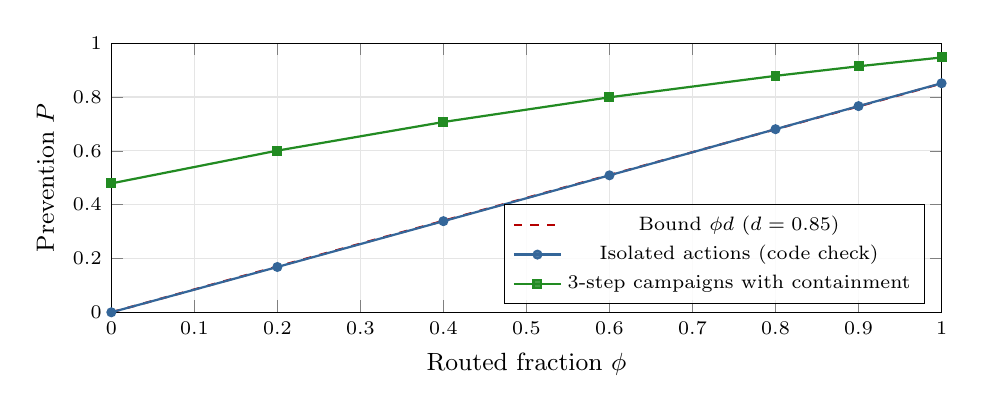
\begin{tikzpicture}
\begin{axis}[width=\columnwidth, height=5.0cm, xlabel={Routed fraction $\phi$}, ylabel={Prevention $P$},
  xmin=0, xmax=1, ymin=0, ymax=1, grid=major, grid style={gray!20},
  legend style={font=\scriptsize, at={(0.98,0.03)}, anchor=south east, fill=white, fill opacity=0.85, text opacity=1},
  tick label style={font=\scriptsize}, label style={font=\small}]
\addplot[deepred, dashed, thick] coordinates {(0.0,0.0) (0.2,0.17) (0.4,0.34) (0.6,0.51) (0.8,0.68) (0.9,0.765) (1.0,0.85)};
\addlegendentry{Bound $\phi d$ ($d=0.85$)}
\addplot[steelblue, thick, mark=*, mark size=1.4pt] coordinates {(0.0,0.0) (0.2,0.1684) (0.4,0.3386) (0.6,0.5089) (0.8,0.6803) (0.9,0.766) (1.0,0.8509)};
\addlegendentry{Isolated actions (code check)}
\addplot[midgreen, thick, mark=square*, mark size=1.4pt] coordinates {(0.0,0.4789) (0.2,0.6007) (0.4,0.707) (0.6,0.7988) (0.8,0.8785) (0.9,0.914) (1.0,0.9468)};
\addlegendentry{3-step campaigns with containment}
\end{axis}
\end{tikzpicture}
\caption{Prevention versus the share of actions routed through the gateway. The isolated-action curve reproduces $\phi d$ by construction and serves as a check of the simulation code. When a catch, or an out-of-path alert raised with an assumed probability of 0.6, contains the rest of a three-step campaign, prevention exceeds $\phi d$: the bound of Eq.~(\ref{eq:coverage}) applies to each action separately. Simulated; 10 seeds, 95\% CIs below 0.006.}
\label{fig:simcoverage}
\end{figure}

\textbf{The coverage bound holds per action, not per campaign.} Fig.~\ref{fig:simcoverage} varies $\phi$ for a single in-path detector with $d=0.85$. For isolated actions the simulation computes prevention as the product of routing and detection, so its agreement with $\phi d$ (0.17 at $\phi=0.2$, 0.85 at $\phi=1$) confirms the code rather than the bound. The informative curve is the other one. When attacks arrive as three-step campaigns and a catch or an out-of-path alert contains the rest of the session, prevention exceeds $\phi d$, reaching 0.48 even at $\phi=0$, where nothing is gated. Its exact height depends on the assumed alert probability, but its direction does not: the bound of Section~\ref{sec:hacof}.K describes a single action, and out-of-path containment buys campaign-level prevention that no single gate provides.

\begin{figure}[!t]
\centering
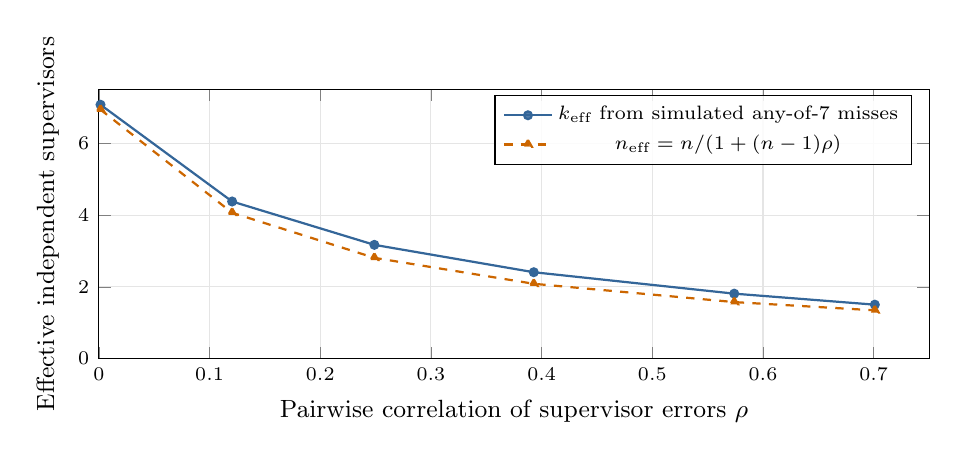
\begin{tikzpicture}
\begin{axis}[width=\columnwidth, height=5.0cm, xlabel={Pairwise correlation of supervisor errors $\rho$}, ylabel={Effective independent supervisors},
  xmin=0, xmax=0.75, ymin=0, ymax=7.5, grid=major, grid style={gray!20},
  legend style={font=\scriptsize, at={(0.98,0.98)}, anchor=north east, fill=white, fill opacity=0.85, text opacity=1},
  tick label style={font=\scriptsize}, label style={font=\small}]
\addplot[steelblue, thick, mark=*, mark size=1.4pt] coordinates {(0.0015,7.074) (0.1204,4.378) (0.2489,3.17) (0.3929,2.407) (0.574,1.81) (0.701,1.503)};
\addlegendentry{$k_{\text{eff}}$ from simulated any-of-7 misses}
\addplot[ambercolor, thick, dashed, mark=triangle*, mark size=1.6pt] coordinates {(0.0015,6.937) (0.1204,4.064) (0.2489,2.808) (0.3929,2.085) (0.574,1.575) (0.701,1.345)};
\addlegendentry{$n_{\text{eff}}=n/(1+(n-1)\rho)$}
\end{axis}
\end{tikzpicture}
\caption{Seven supervisors, each with detection rate 0.7, raising an alarm if any one fires. $k_{\text{eff}}$ is the number of independent supervisors that would give the same joint miss rate; the design-effect approximation of Eq.~(\ref{eq:neff}) slightly underestimates it at every correlation tested. Simulated; one-factor Gaussian error model, 5 seeds of 20{,}000 trials.}
\label{fig:simneff}
\end{figure}

\textbf{The effective-supervisor approximation is conservative here.} Fig.~\ref{fig:simneff} gives seven supervisors a detection rate of 0.7 each and an alarm if any one fires. With independent errors the joint miss rate is about $2\times10^{-4}$; as the measured pairwise error correlation rises to 0.70, it climbs to about 0.16, roughly 750 times higher. Converting each simulated joint miss rate into an equivalent number of independent supervisors gives 4.4, 2.4, and 1.5 at error correlations of 0.12, 0.39, and 0.70; the approximation $n/(1+(n-1)\rho)$ gives 4.1, 2.1, and 1.3. Across the range tested the approximation errs on the cautious side, the direction a design rule should err in. It was, however, derived for averages and does not cover any-of-$n$ alarms, and under a different error structure the gap could change sign.

\textbf{What these results do not show.} The detectors are Bernoulli draws with assumed rates, not language models; the attacker does not adapt to the supervisors; the workload is one agent type with one profile; human approvers and reviewers are modeled by fixed accuracy rates; and parameter values are assumptions chosen to be plausible, not estimates. The simulation can show that \hacof{}'s parts are logically consistent, how its bounds behave, and which parameters drive its costs. It cannot show that real supervisors reach these rates, which is what the protocol of Sections~\ref{sec:eval}.A--C, run with real agents and real models, has to establish.

\subsection{\textcolor{slateblue}{Staged Deployment}}
\label{sec:eval-roadmap}

Deployment proceeds in seven phases, summarized in Table~\ref{tab:roadmap}. Each phase has entry criteria that must hold before it starts and exit criteria, expressed in the metrics of Table~\ref{tab:metrics}, that must hold before the next one begins. The numerical thresholds are deliberately left to Phase~I: an acceptable false-positive rate for an internal document workflow would be reckless for a payments system, and fixing thresholds after seeing results invites the deployer to set them wherever the results happen to fall.

\begin{table*}[!t]
\caption{Staged Deployment Roadmap: Entry Criteria, Activities, and Exit Criteria}
\label{tab:roadmap}
\centering
\footnotesize
\setlength{\tabcolsep}{4pt}
\begin{tabular}{>{\raggedright\arraybackslash}p{2.3cm}>{\raggedright\arraybackslash}p{3.9cm}>{\raggedright\arraybackslash}p{5.0cm}>{\raggedright\arraybackslash}p{5.0cm}}
\toprule
\rowcolor{darkblue!15}
\textbf{Phase} & \textbf{Entry criteria} & \textbf{Key activities} & \textbf{Exit criteria (Table~\ref{tab:metrics} metrics)} \\
\midrule
I.\ Governance definition & named accountable officer and policy owner; legal sources for the deployment identified & map Layer~1 obligations; set risk classes; fix per-category thresholds for every metric; define the appeal path and its deadlines & every planned rule has a clause source; thresholds recorded and signed before any test \\
\rowcolor{darkblue!5}
II.\ Policy engineering & Phase~I signed off & write authorization profiles and boundary rules; build test suites from the ten scenario families & every profile passes its tests; \textit{audit completeness} target met on synthetic decisions \\
III.\ Technical integration & profiles approved & deploy identity, gateways, transaction holds, and the audit plane; connect telemetry & every governed action produces a record; \textit{audit completeness} met on live traffic; gateway fails closed in outage drills \\
\rowcolor{darkblue!5}
IV.\ Supervisory monitoring (observe-only) & Phase~III exit met & run Agents A--G without enforcement; build per-agent baselines; seed known violations & \textit{false-positive rate}, \textit{violation detection rate}, and \textit{mean time to detection} measured per risk category with uncertainty intervals; baselines approved \\
V.\ Controlled enforcement & Phase~IV evidence meets the Phase~I false-positive thresholds & switch on automated denial only for scenarios that passed testing; route everything ambiguous to people & \textit{prevention effectiveness}, \textit{mean time to containment}, \textit{residual harm}, and \textit{review and appeal outcomes} within thresholds \\
\rowcolor{darkblue!5}
VI.\ Independent assurance & Phase~V stable over the agreed observation period & red-team exercises against agents and supervisors; privacy impact review; security audit; measurement of supervisor reliability and of $\rho$ (Section~\ref{sec:hacof}.K) & external auditor's report filed; \textit{privacy impact} within limits; supervisor diversity confirmed by ablation \\
VII.\ Continuous improvement & Phase~VI report accepted & approved, regression-tested policy and baseline updates; periodic re-assurance & no update raises the \textit{false-positive rate} or lowers \textit{violation detection rate} beyond threshold; \textit{recovery time} tracked \\
\bottomrule
\end{tabular}
\end{table*}

Phase~IV is the phase most likely to be skipped and the one that matters most. It is where the deployer learns what its supervisors flag when nothing is being enforced, and it produces the false-positive evidence on which the decision to enter Phase~V depends; a deployment that moves straight from integration to enforcement is setting thresholds by guesswork. Pilots should start in bounded, reversible settings (an internal document workflow, say, before a payments system) and move outward only when a phase's exit criteria are met. Pakistan's planned regulatory sandbox (Section~\ref{sec:case}.D) is the kind of setting Phases~I--IV suit. If a phase fails its own criteria, the deployment steps back one phase rather than forward, and the failure is recorded as a result in its own right under the reporting requirements above.

\section{\textcolor{darkblue}{Limitations}}
\label{sec:limits}

Several of these limitations are load-bearing. Readers should weigh them before generalizing the framework.

\textbf{Single-case-study generalizability.} Pakistan is one country with a particular colonial-administrative legal tradition, a particular ICT export profile, and a particular dependence on foreign capital that does not transfer cleanly to an economy with different trade dependencies. We do not test the four-pillar profile against other non-major economies' national policies, so the claim that Pakistan's profile is structural rather than idiosyncratic rests on the resource argument of Section~\ref{sec:framework}, not on cross-country evidence. The four-pillar structure likely generalizes; the specific numbers in Section~\ref{sec:case}.B do not, and this paper makes no claim that they do.

\textbf{Policy documents date quickly.} Pakistan's National AI Policy was current as of its 2025 publication; funding figures, institutional staffing plans, and even the EU AI Act's implementation timeline described in Section~\ref{sec:background}.A are all subject to revision on a timescale shorter than a journal's publication cycle. A reader checking any cited figure against the live source should expect the figure to have moved since publication, which does not by itself make it wrong.

\textbf{No primary interviews or surveys were conducted.} Every empirical claim in Sections~\ref{sec:background}, \ref{sec:framework}, and~\ref{sec:case} rests on published policy documents, funding disclosures, and secondary labor-market data, and Section~\ref{sec:hacof} is a design proposal built on published technical work. None of it rests on original survey or interview data with regulators, AI lab staff, or displaced Pakistani IT workers. A primary-data study specifically testing whether regulators inside the three major powers themselves perceive the capacity asymmetry described here would be a stronger empirical test than this paper can offer on its own.

\textbf{Asymmetric data availability biases the comparison itself.} The three major powers publish far more granular data about their own regulatory institutions --- staffing counts, budget lines, enforcement actions --- than most non-major economies publish about theirs. Table~\ref{tab:comparison} is, by necessity, built on richer evidence for the first three columns than the fourth, which means the comparative gap this paper documents may partly measure what gets published more than what exists. This bias most likely understates the non-major-economy column, since evaluators tend to treat missing data as missing capacity, but the paper cannot rule out the reverse.

\textbf{The four-pillar framework itself has not been empirically validated against governance outcomes.} We argue the framework from first principles and illustrate it with one detailed case. It does not test whether a government scoring high on all four pillars actually produces measurably better AI-safety outcomes than one scoring low --- that causal link is assumed by analogy to how capacity operates in other regulatory domains; it is not demonstrated with outcome data specific to AI governance. No AI-governance regime has existed long enough to generate the outcome data such a test would require, which is itself part of why no other methodology has closed this gap.

\textbf{\hacof{} is tested only in simulation, and its prevention guarantee is only as wide as its enforcement points.} Section~\ref{sec:eval}.D reports a prototype of the enforcement plane and a simulation whose supervisor rates are assumed rather than measured; it is not a field evaluation, and the full protocol with real agents and models remains to be run. Even if the architecture performs as designed, monitors will miss behavior that is novel, deliberately concealed, spread thinly across many agents, or simply poorly instrumented. In-path gateways stop only the actions routed through them. A vulnerability in the gateway, an enforcement point someone forgot to place, or a privileged account compromised upstream all bypass Layer~3 without tripping it.

\textbf{The supervisors carry their own weaknesses and costs.} Supervisory agents built on language models inherit those models' failure modes, and independence engineered on paper may still leave shared blind spots in practice~\cite{kim2025correlated}. % CLAIM: errors of different LLMs are correlated (Kim et al.), so supervisors may share blind spots.
An adversary who learns how the monitors work can tune an attack to them. Continuous oversight also costs compute and adds latency to every gated action, and the telemetry it requires is itself a store of sensitive data that must be protected and eventually deleted. For a small deployer in a low-income economy, these costs may be large enough to tempt partial adoption, which risks leaving the paperwork of \hacof{} without the protection.

\textbf{Some disagreements are not engineering problems.} What counts as harm, how much risk is acceptable, and whose authority is legitimate are contested questions that no architecture settles; \hacof{} assumes Layer~1 has answered them through lawful institutions, and where those institutions are weak or captured the architecture enforces whatever they decide. Deployments that cross organizations or borders add coordination problems that this paper names but does not solve: interoperable profile formats, allocation of responsibility, cross-border evidence sharing, and outright conflicts between national laws.

\textbf{English-language and Western-source bias in the evidence base.} Pakistan's own Urdu-language policy debate, parliamentary committee discussion, and domestic tech-press coverage of the National AI Policy are not represented in this paper's evidence base, which draws overwhelmingly on English-language government documents, international reporting, and donor and multilateral publications. A debate conducted substantially in Urdu inside Pakistan's own policy community may contain objections, nuances, or planned revisions that English-language sourcing cannot surface.

\section{\textcolor{darkblue}{Conclusion}}
\label{sec:conclusion}

\hacof{} assembles legal authority, machine-readable policy, preventive controls placed outside the model, supervisors kept independent of the agents they watch, live monitoring, early containment, human review, and continuous improvement into one architecture. The reason to assemble them is to move governance off the page and into the systems agents run on: a policy document beside a deployment changes nothing an agent can do, while a gate in front of it does. Under \hacof{}, an agent's authority is sized to its approved purpose, its actions are watched by mechanisms proportionate to the risk, violations meet responses agreed before they happen, and the supervisors themselves stay auditable by, and answerable to, people with legitimate authority. Instructing a model to behave well is the weakest version of this. The stronger version is an environment that makes good behavior the default, blocks forbidden actions wherever a gate can reach them, catches and contains harm that gets past the gates, and keeps a record from which failures of governance itself can be investigated and repaired.

Meaningful human control over AI is not a property a law can declare into existence. It requires boundary-setting authority backed by real enforcement leverage, incentive-steering capital large enough to move a market, HITL regulatory institutions staffed with people who can keep pace with deployment cycles, and algorithmic auditing access to the models being governed. We have argued that all four currently concentrate inside three jurisdictions, and that a government outside them cannot close the gap by legislating harder. That holds for Pakistan, examined here in detail, and by structural extension for most of the more than 70 governments that have issued a national AI strategy. Meaningful participation for a non-major economy requires, at minimum, a market-access or coalition-based lever strong enough to make boundary-setting enforceable against foreign vendors, and a funding commitment that matters at least regionally. It also needs a technical staffing pipeline built for AI oversight, not borrowed from general ICT regulation, and an audit-access arrangement secured by negotiation or treaty, so that oversight no longer rests on vendor self-reporting.

Capacity at the level of the state is necessary but not sufficient. The second half of the argument is operational. \hacof{} shows what has to exist at the point where an agent acts: authority traced to law, enforcement points the governed model cannot reach, supervisors that are themselves supervised, and monitoring confined to AI activity rather than people. Its mapping onto the pillars yields a practical asymmetry. A low-capacity state cannot audit a foreign model's weights, but it can require domestic deployers to keep an audit trail it is able to read, which is a far smaller technical task. That does not close the gap this paper documents; it narrows the part of it a government can act on this budget cycle.

The gaps are not equally pressing, and the agenda below takes them in order.

Audit-access mechanisms for non-major economies are the most urgent gap. No treaty framework, mutual-recognition arrangement, or technical standard currently exists for a government outside the three major powers to obtain independent, verifiable access to a foreign-hosted model's behavior. Nothing here needs new money so much as a protocol that does not yet exist: a negotiated technical-access protocol that a coalition of non-major economies could plausibly demand jointly even without any single member having individual leverage. International financial auditing offers a rough structural precedent worth studying, though not copying wholesale: authorities responsible for globally active banks rely on cross-border cooperation arrangements and shared standards because no single national authority can resolve such a bank unilaterally~\cite{baselcommittee2010crossborder}.
The analogy is imperfect, because banks are heavily regulated at origin in a way frontier AI labs currently are not, but the underlying mechanism, pooled technical standards substituting for individual enforcement power, is the right shape of solution to study first.

Coalition-based boundary-setting leverage is a different kind of problem, and treating it like the audit-access gap would misdiagnose both. A single mid-sized economy's market is not large enough to compel vendor compliance, but a bloc of such economies negotiating jointly, on the model of regional trade blocs that already pool market access for other purposes, plausibly is. This requires institution-building that outlasts any single government's term, coordination costs that regional organizations historically struggle to sustain, and a shared technical baseline for what ``compliance'' even means across member states with different legal traditions. It is a harder, slower project than the audit-access mechanism above, and that is why it should not be allowed to become the default first target simply because it sounds more comprehensive.

A validated empirical test of the four-pillar framework against actual governance outcomes must come before any policy recommendation that claims a given capacity investment will causally improve AI-safety outcomes, not merely the framework's own capacity score. Until it exists, this framework should be read as a diagnostic structure whose predictions are not yet certified. The same discipline applies to \hacof{}: the protocol of Section~\ref{sec:eval}, and in particular its ablation testing whether seven supervisors built on one base model behave as one, should be run before any regulator writes \hacof{}-style requirements into binding rules.

The remaining items --- primary survey data on regulator and displaced-worker perspectives, country comparisons beyond the single Pakistani case, and interoperable formats for authorization profiles and audit records across jurisdictions --- matter, but they extend the evidence base, and they can proceed in parallel with the three items above; they need not wait for them.

The guiding principle of \hacof{} is the one we close on: AI should be developed and operated for the benefit of humanity, under enforceable rules that people define, with continuous technical oversight and accountable authority over both the systems being governed and the systems that govern them.

\section*{\textcolor{darkblue}{Acknowledgments}}

This work received no external funding or institutional support.

The text of Sections I--IX was drafted with the assistance of Claude (Anthropic), an artificial intelligence system, which provided literature research assistance, drafting assistance, fact-checking assistance, and assistance in writing the prototype and simulation code of Section~VII-D under the direction, review, and final verification of the author, who is fully accountable for all content, citations, and claims in this article. No AI system is credited as an author.

\bibliographystyle{IEEEtran}
\bibliography{references}

\end{document}
